\chapter{Implementation}

\section{Web Application}
The application consists of a front end, API for connecting to the ajax calls for loading more messages in a chat box, web sockets and the main back end. The application was built from a few languages, Python for the back end and HTML, CSS, and JavaScript/jQuery for the front end, with JinJa2 as the tempting engine, used by Python Flask to inject elements from the back end to the front end. The application was built using the Flask framework.

The Flask template \cite{flask_template_mine} used was built last year after building multiple web projects to prevent the need for the repetitive setup every time a new Flask project is created. The template comes built with a basic setup for a web app which includes: Register/Login functionality with a user module ready for committing to the database and basic routes/views such as home, contact, about and 404 pages predefined.  

After importing the template, it was converted from a single app structure to use blueprints for separating out the different parts of the application, such as social, module, user sections, etc. The Flask-migrations module was added to manage changes to the database structure and improve maintainability.

A configurations file (config.py) was used to store the passwords and settings for the application infrastructure such as the database URI, secret key, Imagekit private key, etc. An example of the config file is below:

\begin{lstlisting}
    from datetime import timedelta
    remember_cookie_duration=timedelta(days=<- int days ->)
    secret_key='mvoew0iurpon34jfmxnf4oi'
    debug_setting=True
    sqlalchemy_track_modifications=False
    
    # database uri
    database_uri='mysql+pymysql://
        <- DB Username ->:<- DB Password ->@
        <- DB domain or IP (localhost normally) ->
        /<- DB Name ->'
    
    ## uploading files
    # Image Kit SDK initialization
    imagekit_private_key='private_/LcJLnAbb0x58/smmwjI9NlakB0='
    imagekit_public_key='public_EpuGYME8CyHn7iwcbm1pC0iJ7NY='
    imagekit_url_endpoint='https://ik.imagekit.io/p6la6tqvk'
    
                       #MB * KB * B
    max_content_length=5 * 1024 * 1024 # 5 MB # 5242880
    # for picking useable extensions: 
        https://docs.imagekit.io/api-reference/upload-file-api
    image_extensions=['png', 'jpg', 'jpeg', 'gif']
    document_extensions=['pdf']
    
    user_code='pjfkjfiejfhfoiewfue9fu09fueg'
    admin_code='i98mg807976758r0c098cn847r97'

\end{lstlisting}

\subsection{Flask verses Django}
Originally Django was the chosen framework to be used as it has become the industry standard choice for using Python as a back end. Django offers many of the same capabilities as Flask except, Django comes pre-built with a lot of the tools one would need to develop a production-ready application. Django has an ORM (Object Relational Mapping) used for interacting with the database, a templating engine and more built-in whereas Flask comes with non of that. 

Flask needed modules to be added to gain this extra functionality. For example, to gain an ORM in Flask, flask-sqlalchemy needed to be added which uses sqlalchemy, making it play nice with Flask, and adding some extra functionalities on top.


\subsection{Languages}

\subsubsection{Python}
Flask was the framework of choice which uses Python. This was due to the knowledge from using to build other applications during the university course and from personal projects.

\subsubsection{HTML + CSS}
HTML and CSS were used to style and structure the front-end. JinJa2 is the tempting engine used by Flask for injecting elements from the back-end into the front-end on the server before it is pushed to the client. Bootstrap was also used for styling the application as it allows for quick styling of elements on the front-end.

\subsubsection{JavaScript}
JavaScript and jQuery were used for some front-end applications such as connecting the WebSockets on the back end to the front-end. They were also used to connect to the API for requesting new messages on loading the single module pages and single message pages.


\section{Database}

\begin{figure}[H]
\centering
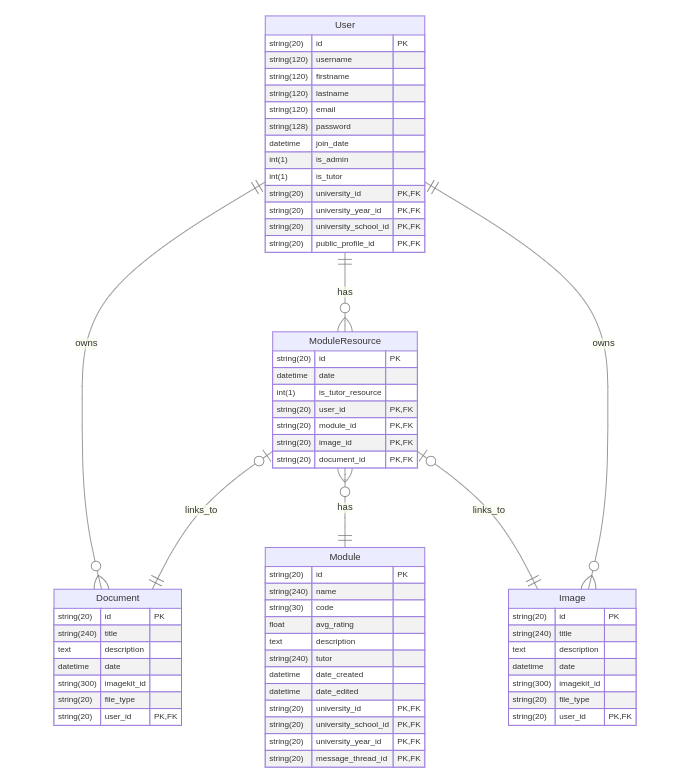
\includegraphics[scale=0.35]{images/database/db_module_resource.png}
\caption{Database class diagrams relevant to module resources}
\label{fig:figure2}
\end{figure}

\begin{figure}[H]
\centering
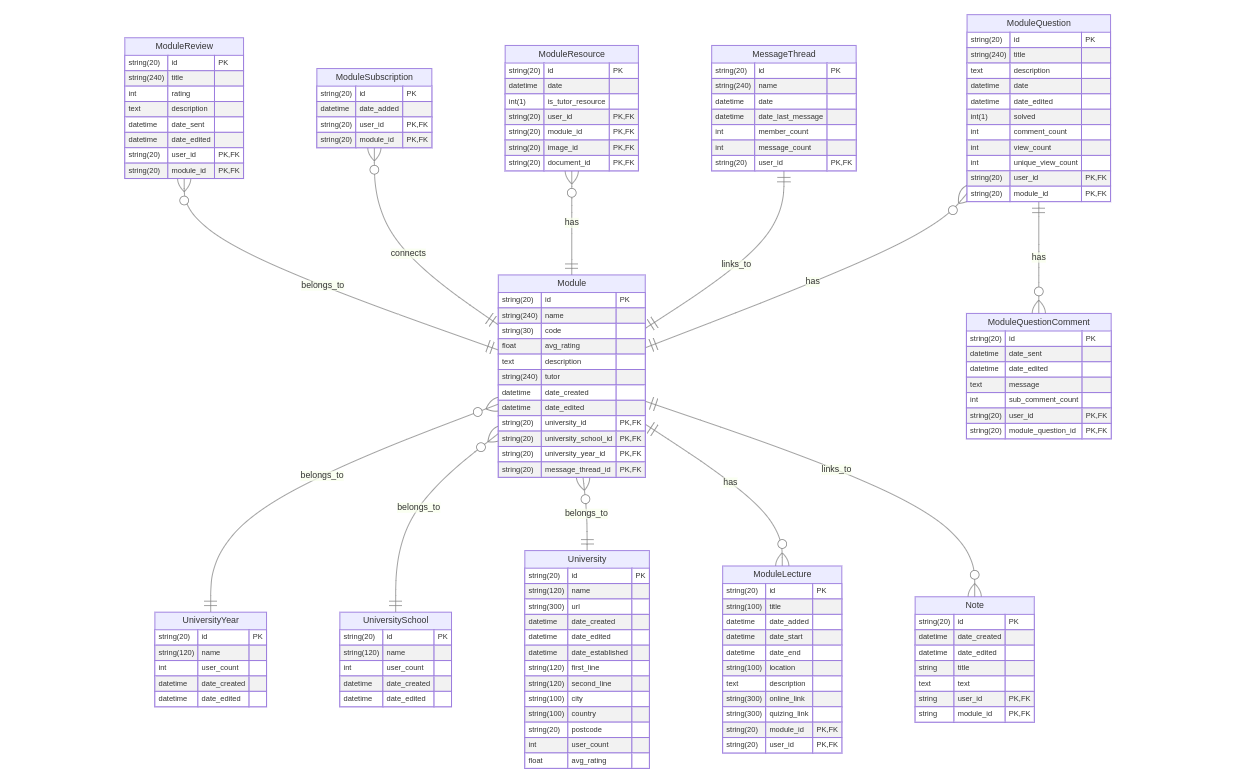
\includegraphics[scale=0.35]{images/database/db_module.png}
\caption{Database class diagrams relevant to modules}
\label{fig:figure2}
\end{figure}

\begin{figure}[H]
\centering
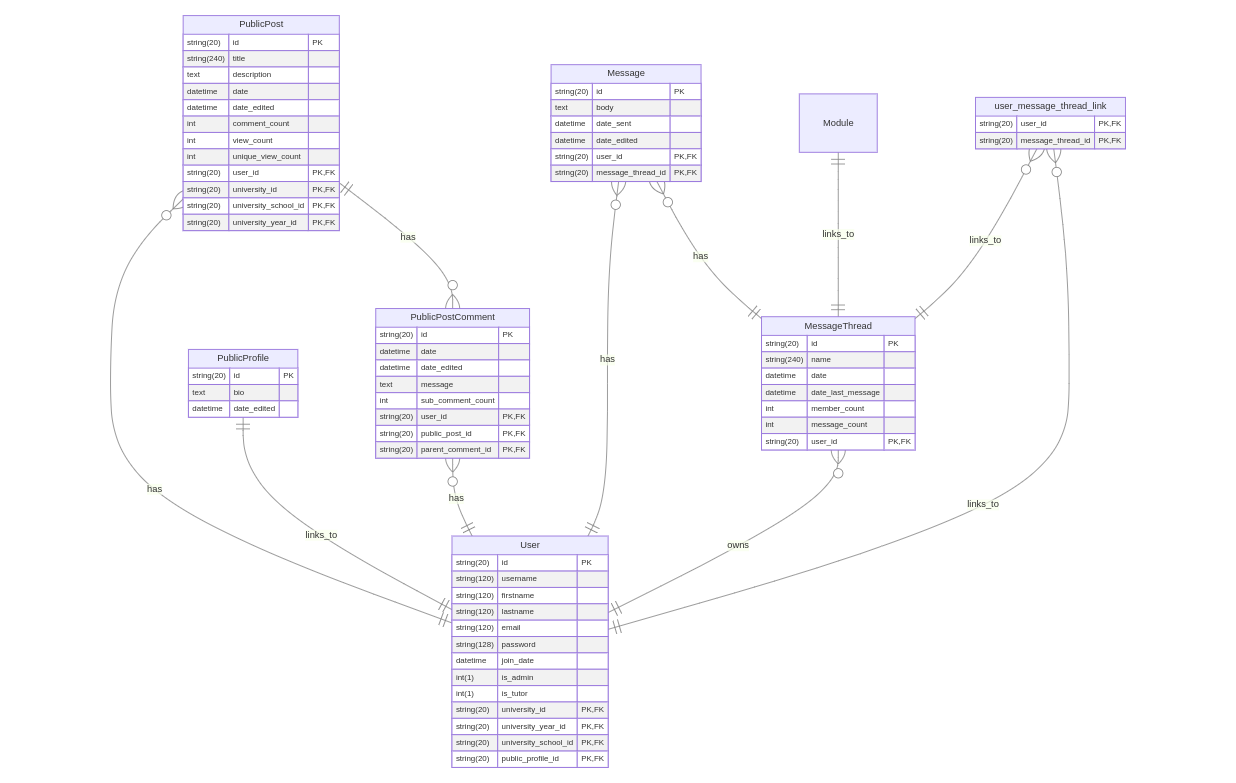
\includegraphics[scale=0.30]{images/database/db_social.png}
\caption{Database class diagrams relevant to social elements of the application}
\label{fig:figure2}
\end{figure}

\begin{figure}[H]
\centering
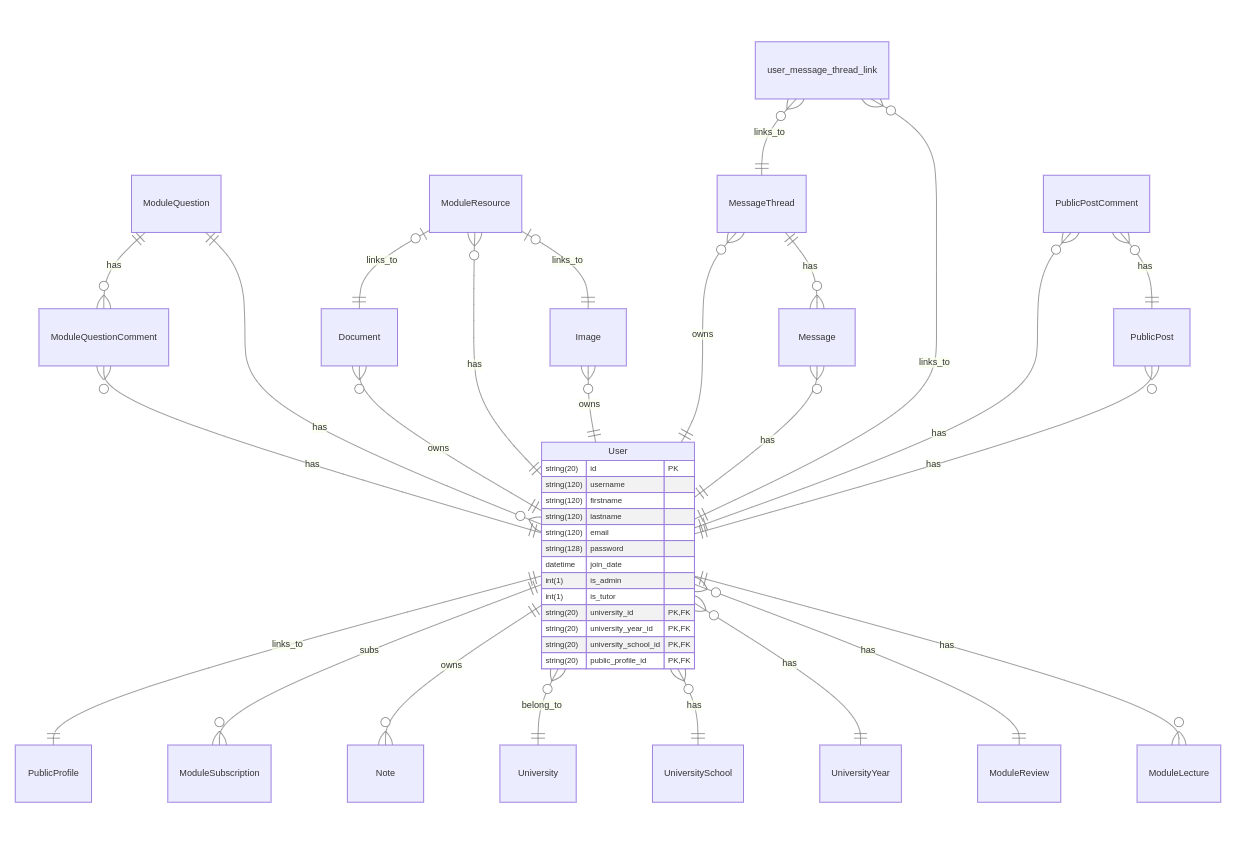
\includegraphics[scale=0.30]{images/database/db_user.png}
\caption{Database class diagrams relating to a user}
\label{fig:figure2}
\end{figure}

\section{Deployment and System Architecture}
Hosting the prototype application had two main options: deploying to a cloud solution like AWS or to a bare metal server located at home. Deploying the application on a Bare metal server meant full control and simplicity with less of a learning curve. However, deploying to AWS meant salability in the long term, despite the added complexity and the ability to learn a new skill. AWS was the final choice used for hosting the application due to scalability and the valuable learning experience. But the main reason was that an application hosted on AWS was less likely to fall victim to someone accidentally turning off the power when testing and demonstrating compared to a server located in a shed in a personal residence.


\begin{figure}[H]
\centering
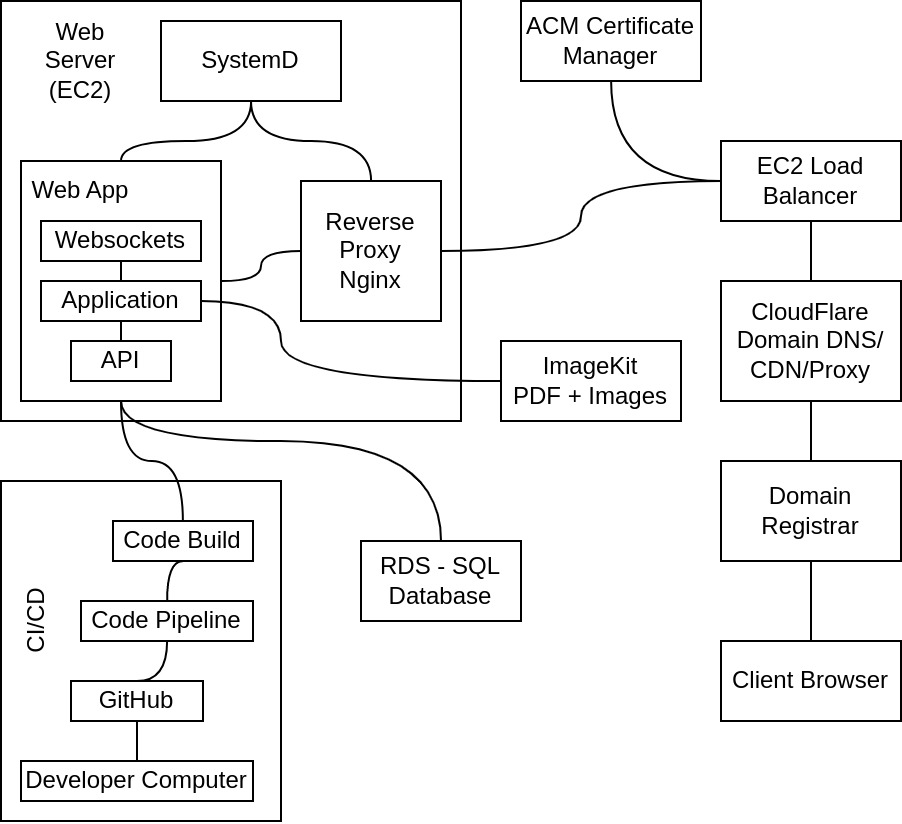
\includegraphics[scale=0.30]{images/architecture_diagram.jpg}
\caption{Final application architecture diagram}
\label{fig:figure2}
\end{figure}

\subsection{Bare metal hosting}
A shared hosting solution was used for past products and coursework, but due to the recent acquisition of some second-hand servers, the opportunity to deploy the application at home became an option. With bare metal hosting, the option was to use an HP DL380 Gen8/9 at home with either Ubuntu 20.04 deployed directly onto the server or, more likely, deployed into a Proxmox MV (Virtual Machine). As Proxmox has the convenience of accessing/interacting with the instance in a browser, it adds some extra flexibility.

To make accessing the application from a personal residence secure (with respect to a home network) Cloudflare tunnelling would be used as the solution, which means the domain is pointed to Cloudflare \cite{cloud_flare}, then use tunnelling to connect to the server inside the network without exposing any ports (which would have been done using port forwarding) to the outside world. This reduces the risk to the network of any way easily penetrating through and gaining access to the server (or any other device). By using Cloudflare, the benefit of DOS protection is also included for protecting the server, reducing a false load.

\subsection{Servers on AWS}
Elastic Beanstalk (EB) was the original choice for deploying the application, as it allows for an application built in languages such as Python, Ruby, JavaScript, etc, to be deployed with one click and minimal configuration. It was set up so that when code is pushed to the main branch on GitHub, it is detected by AWS Code Pipeline and then redeployed to the EB automatically. From initial tests of the application deployment,  EB worked well, successfully deploying and running the application.  EB is a very nice tool to use as it is simple to deploy and comes with scalability out of the box, but this simplicity ultimately ended up becoming a problem. EB is designed for simple HTTP applications where a request is sent to it, and a response is returned to the client. Applications such as APIs and normal dynamic or static websites are a perfect fit for EC, but when trying to add more complexity with persistent connection, EB brakes and is unable to handle protocols like WebSockets and RTC.

After the deployment of the full application with WebSockets integrated, using EB became a problem, with many hours wasted. The final deployment dropped EB and switched to deploying directly onto an AWS Elastic Compute Cloud (EC2) as shown in the diagram above.

To handle the job of storing resources such as PDF, DOCX (Word), PPTX (PowerPoint), JPG/JPEG and PNGs shared by users, AWS Simple Storage Service (S3) as initially considered. but as this is an MVP, it was decided against as it was unnecessary for proof of concept.

Instead of using S3 with a larger file type range allowed, ImageKit was used instead. Image kit allows for images, txt files and pfds which for a proof of concept, it was decided that pdfs and images were enough. In future versions, AWS S3 would be used to allow tutors to upload a wider range of file types and to allow students to share doc files as well as pdfs.

Imagekit has powerful and useful API features specifically designed for serving images on the web. ImageKit gives me the ability to easily sort images uploaded to the site and easily include them on a page using only a URL. There is also the ability to transform/translate such as requesting a specific size for the image when requesting the image (in the URL) and all the processing of the image is done automatically before being sent to the client.

\section{PWA verse native app}
There are two main ways to develop and deploy mobile device applications: PWAs (Progressive Web Apps) and developing an app for mobile devices (either as a cross-platform app using a language like Flutter or building native apps for both IOS and Android). Both ways of deploying an app come with their advantages and disadvantages.

\subsection{For apps store based applications}
Developing an app to deploy and be installed on the user's mobile device generally has better compatibility with the inbuilt features and systems of the device. An example is when using the camera on the device can often function better and be easier to interrogate into the app. The biggest issue, and arguably the most important for this application, is the notifications on IOS. Apple still only allows push notifications on IOS devices to be used with native applications that have been downloaded through the Apple app store. PWAs are not able to use this functionality on IOS devices despite Google supporting it for quite a while on modern Android devices.

\subsection{For PWA-based applications}
Dissipate IOS devices not being able to use push notifications, PWAs still have their advantages, especially for quick deployment.

\section{Application pages}

This is only a snapshot of what can be done in the application. For more images of what the application is possible of, refer to the appendix to view all 65 screenshot images of the application.

\begin{figure}[H]
\centering
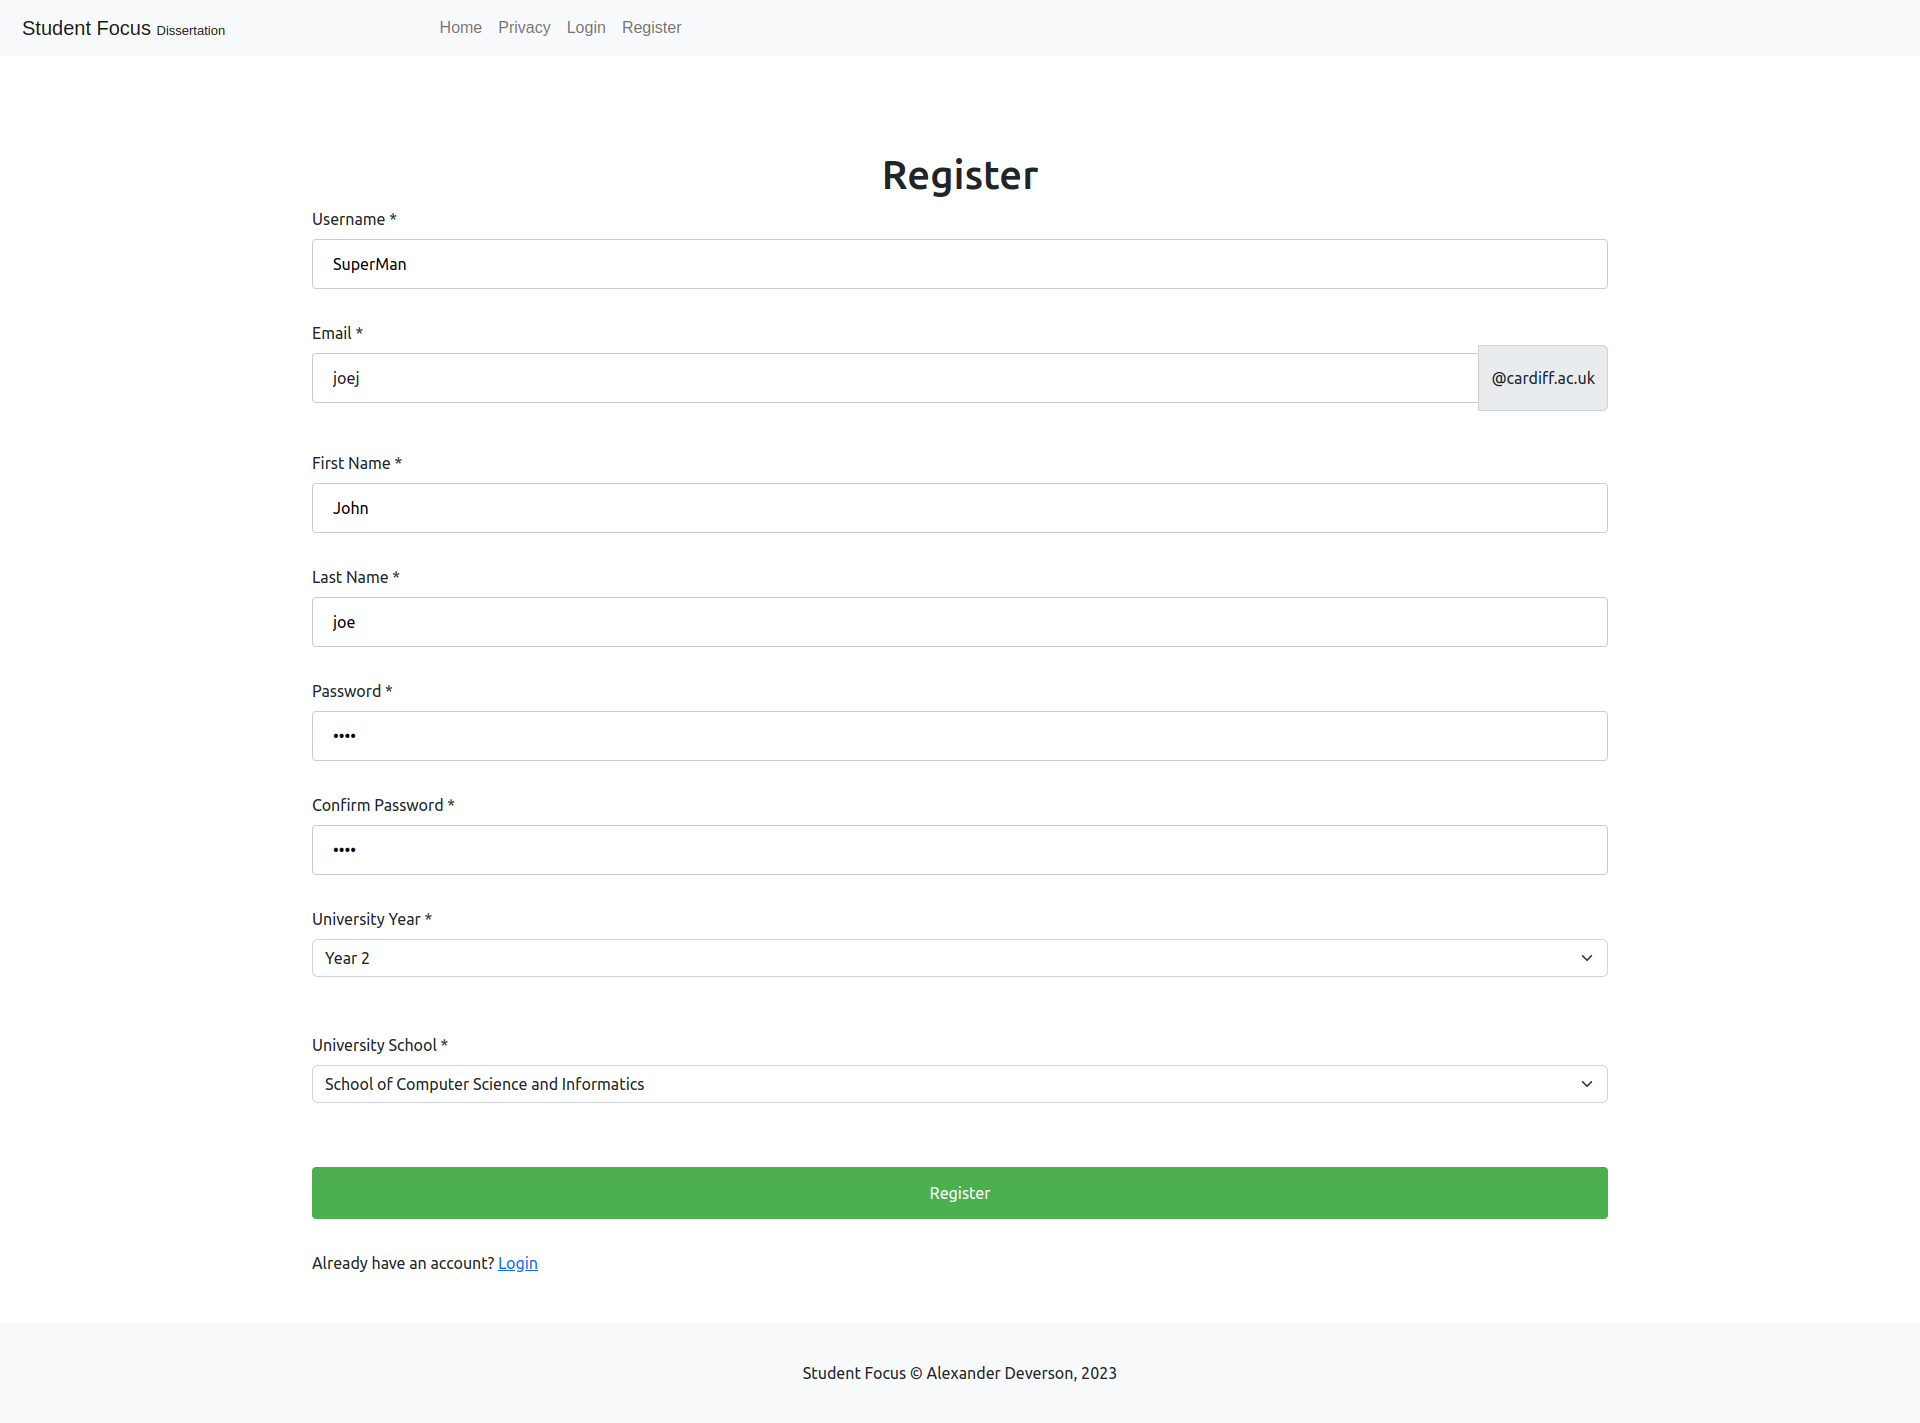
\includegraphics[scale=0.20]{images/application/2 - register_filed_in.png}
\caption{Registration page}
\label{fig:figure2}
\end{figure}

A user can register for the application. If they are a student then they can create an account straight away but if it is for a tutor account then they can create an account, contact the company and the admin can update the user to a tutor on the back end.

\begin{figure}[H]
\centering
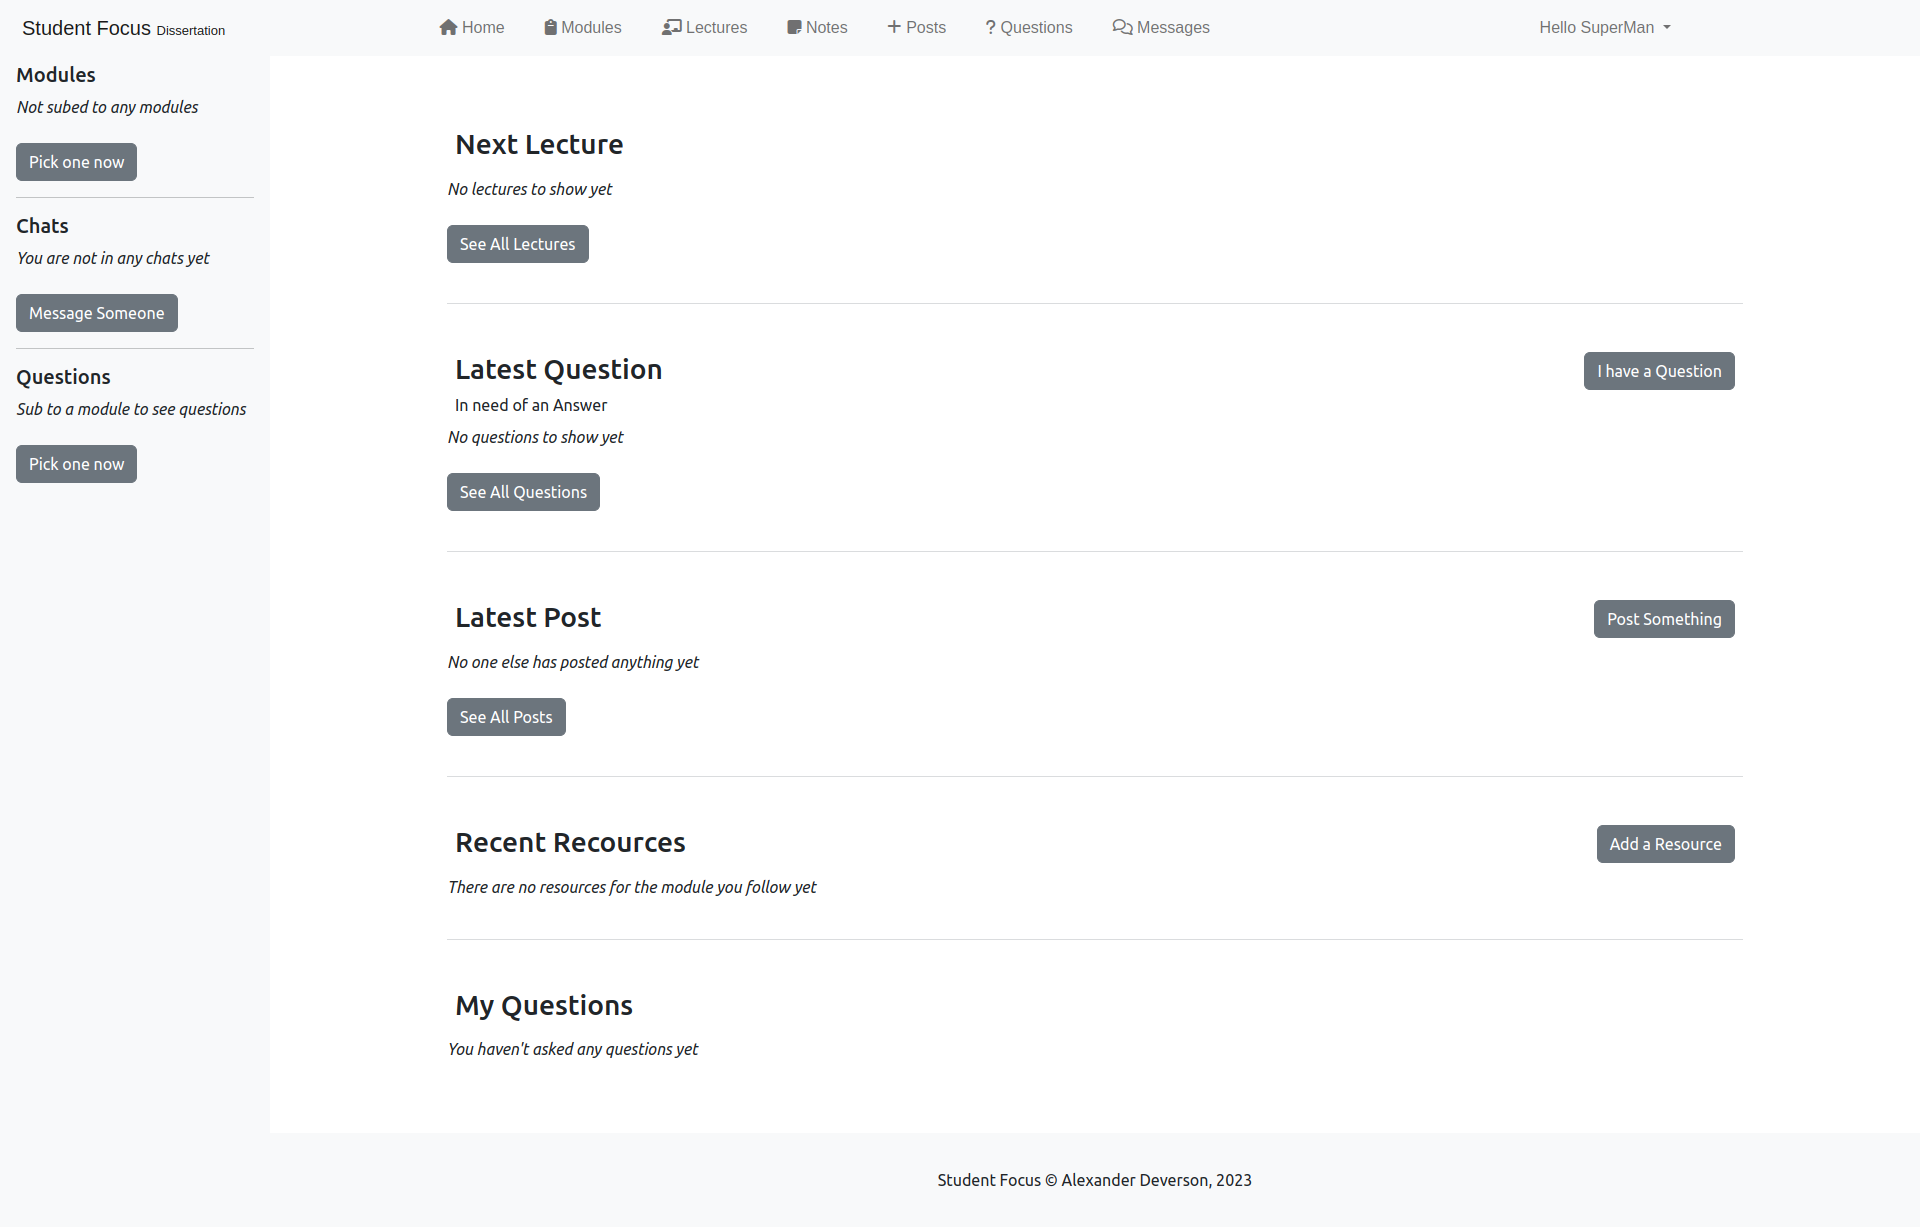
\includegraphics[scale=0.20]{images/application/4 - home_empty.png}
\caption{User's home screen upon first registration}
\label{fig:figure2}
\end{figure}

When the user first registers and logs into the application, they are greeted with their home page which is not populated as they have not subscribed to any modules yet.

\begin{figure}[H]
\centering
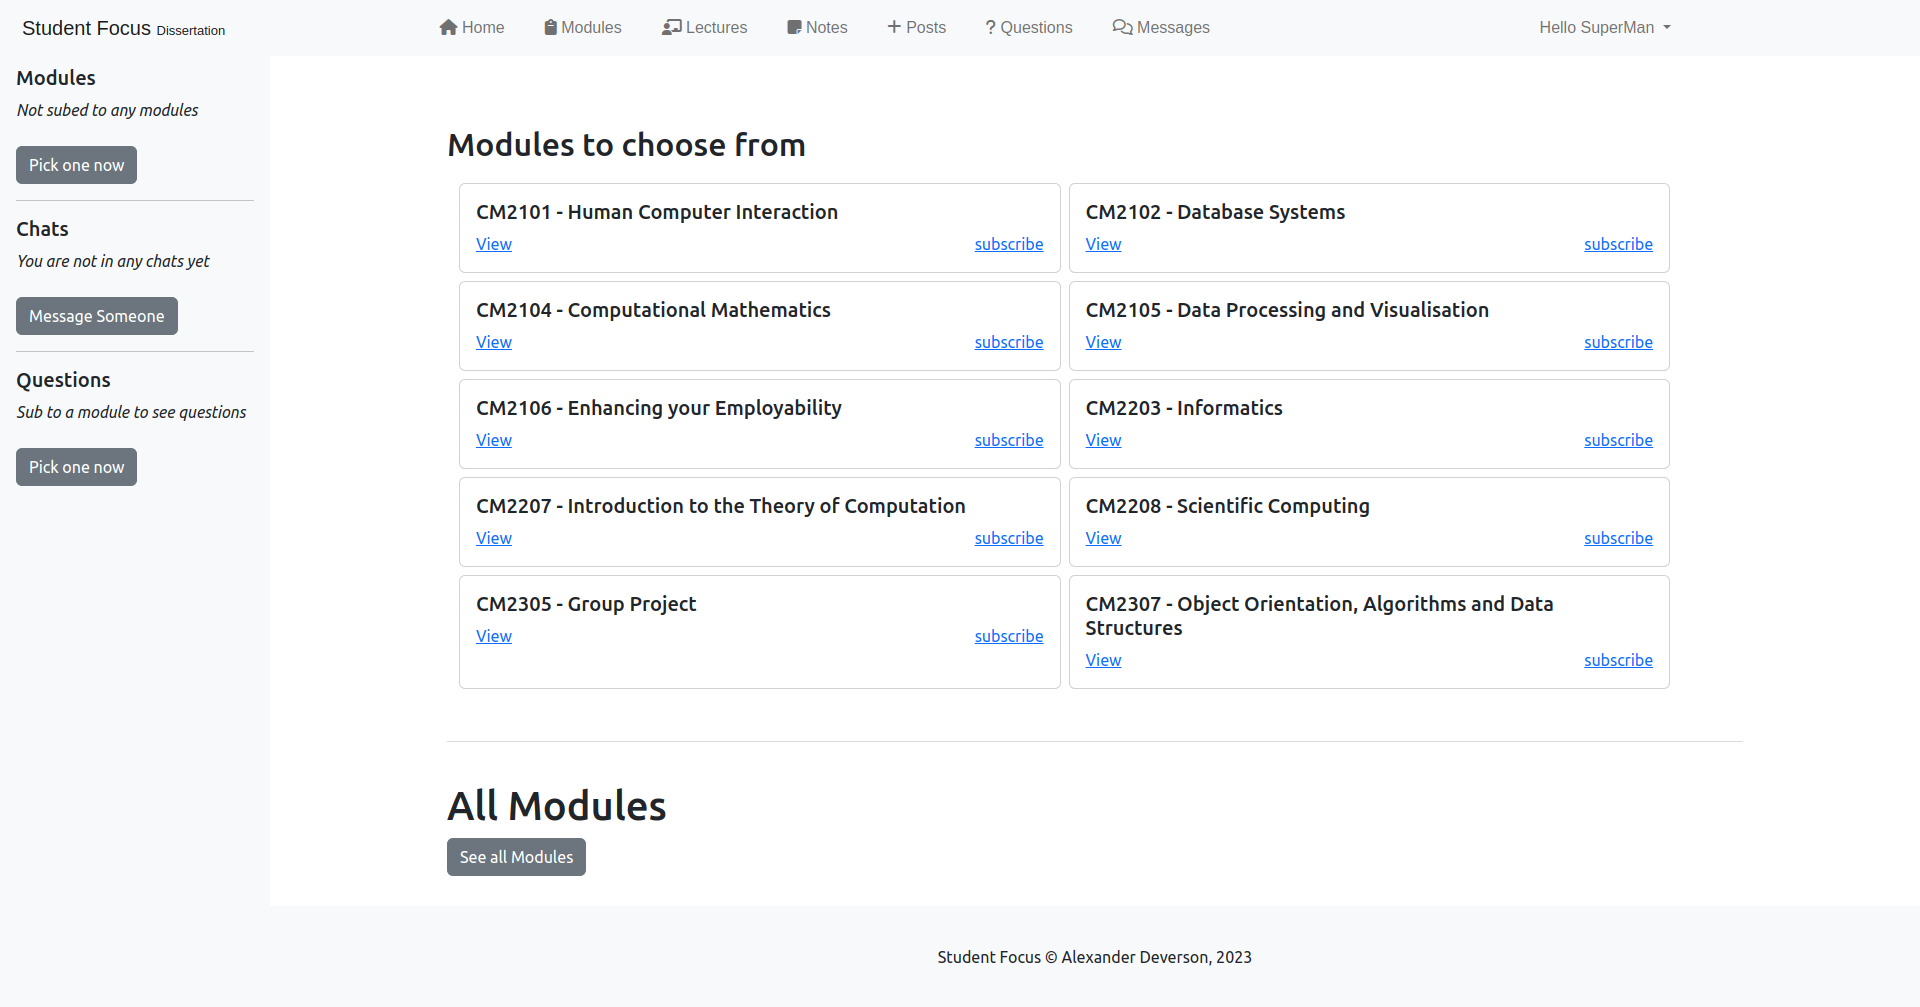
\includegraphics[scale=0.20]{images/application/5 - module_selection.png}
\caption{Module selection page for users}
\label{fig:figure2}
\end{figure}

The user must then pick the modules they are studying.

\begin{figure}[H]
\centering
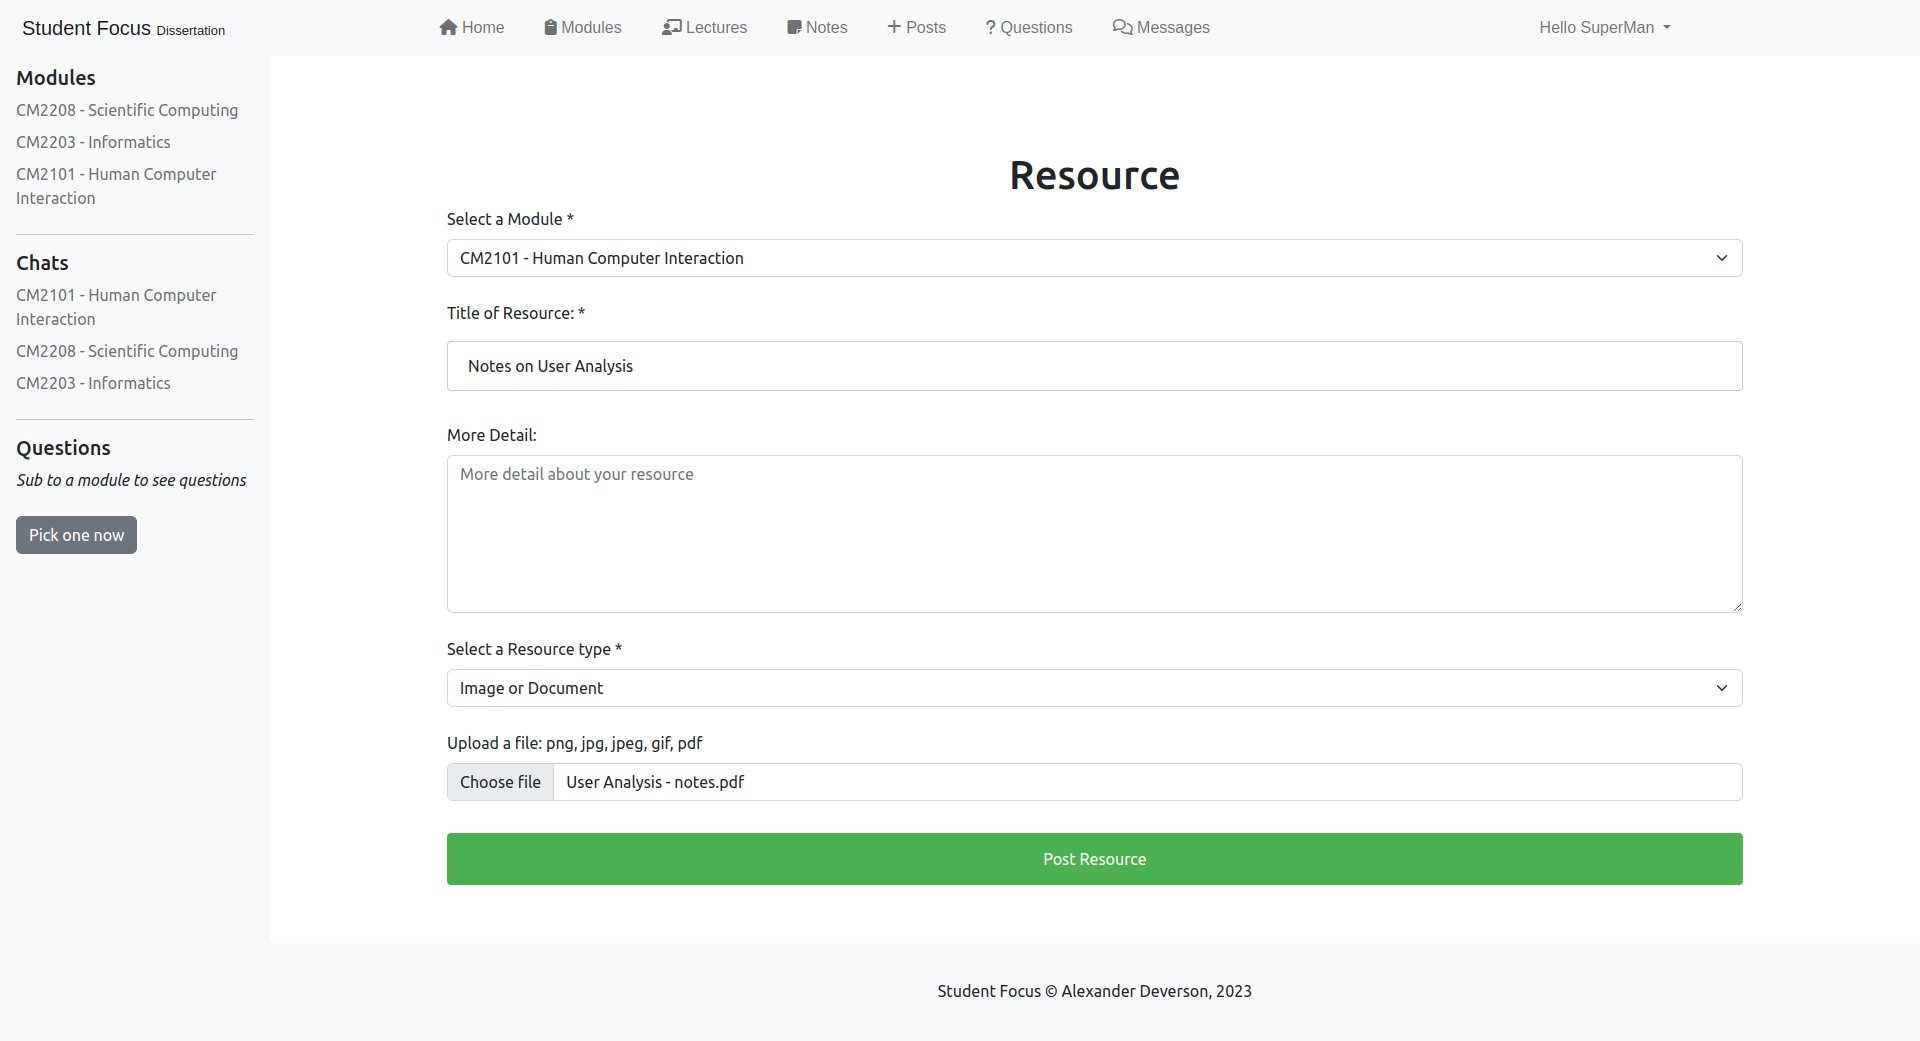
\includegraphics[scale=0.20]{images/application/14 - student resource.png}
\caption{Add new module resource form page}
\label{fig:figure2}
\end{figure}

The user can add resources to a module.

\begin{figure}[H]
\centering
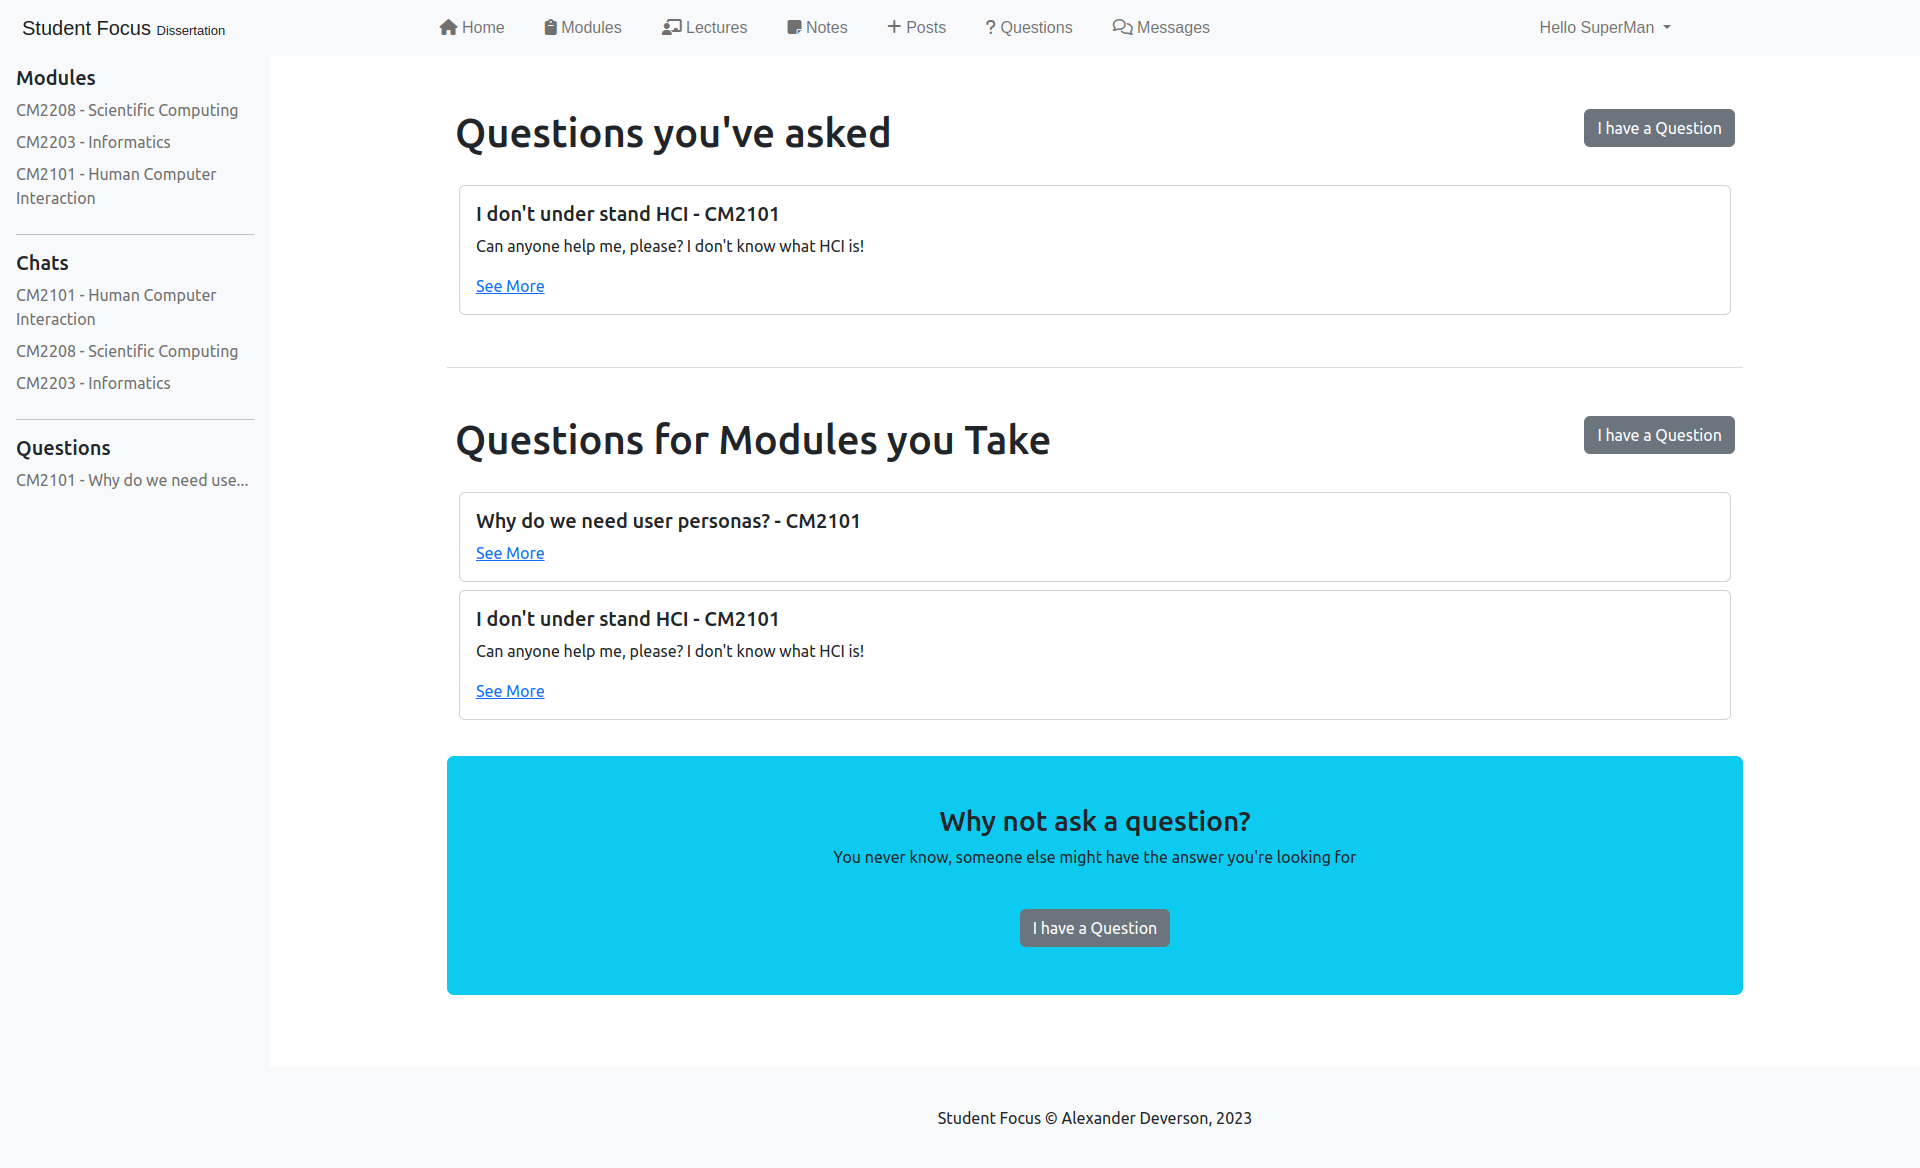
\includegraphics[scale=0.20]{images/application/21 - all_questions.png}
\caption{Module question list page}
\label{fig:figure2}
\end{figure}

Users can view all questions in one place for all the modules they are subscribed to.

\begin{figure}[H]
\centering
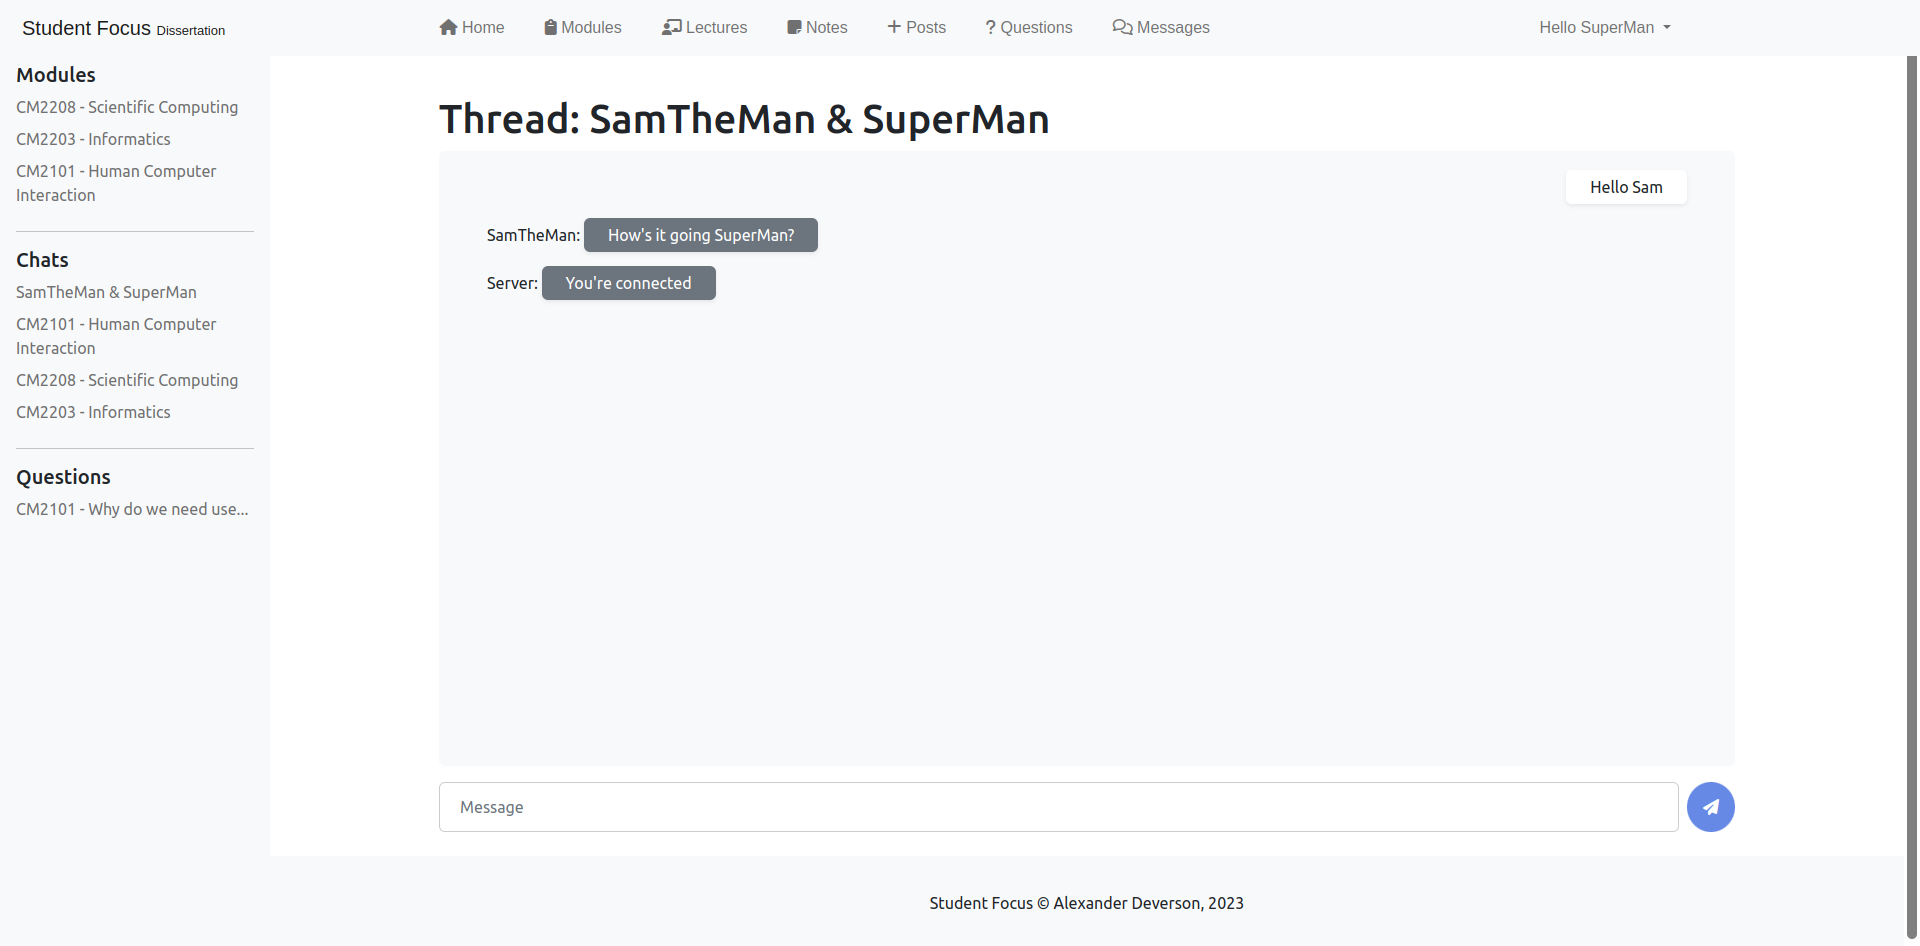
\includegraphics[scale=0.20]{images/application/26 - message_thread_on_refresh.png}
\caption{Other user's profile page}
\label{fig:figure2}
\end{figure}

Users can send messages to each other engaging in conversation in real-time. This is done due to the power of WebSockets establishing a persistent connect between the browser client and the server.

\begin{figure}[H]
\centering
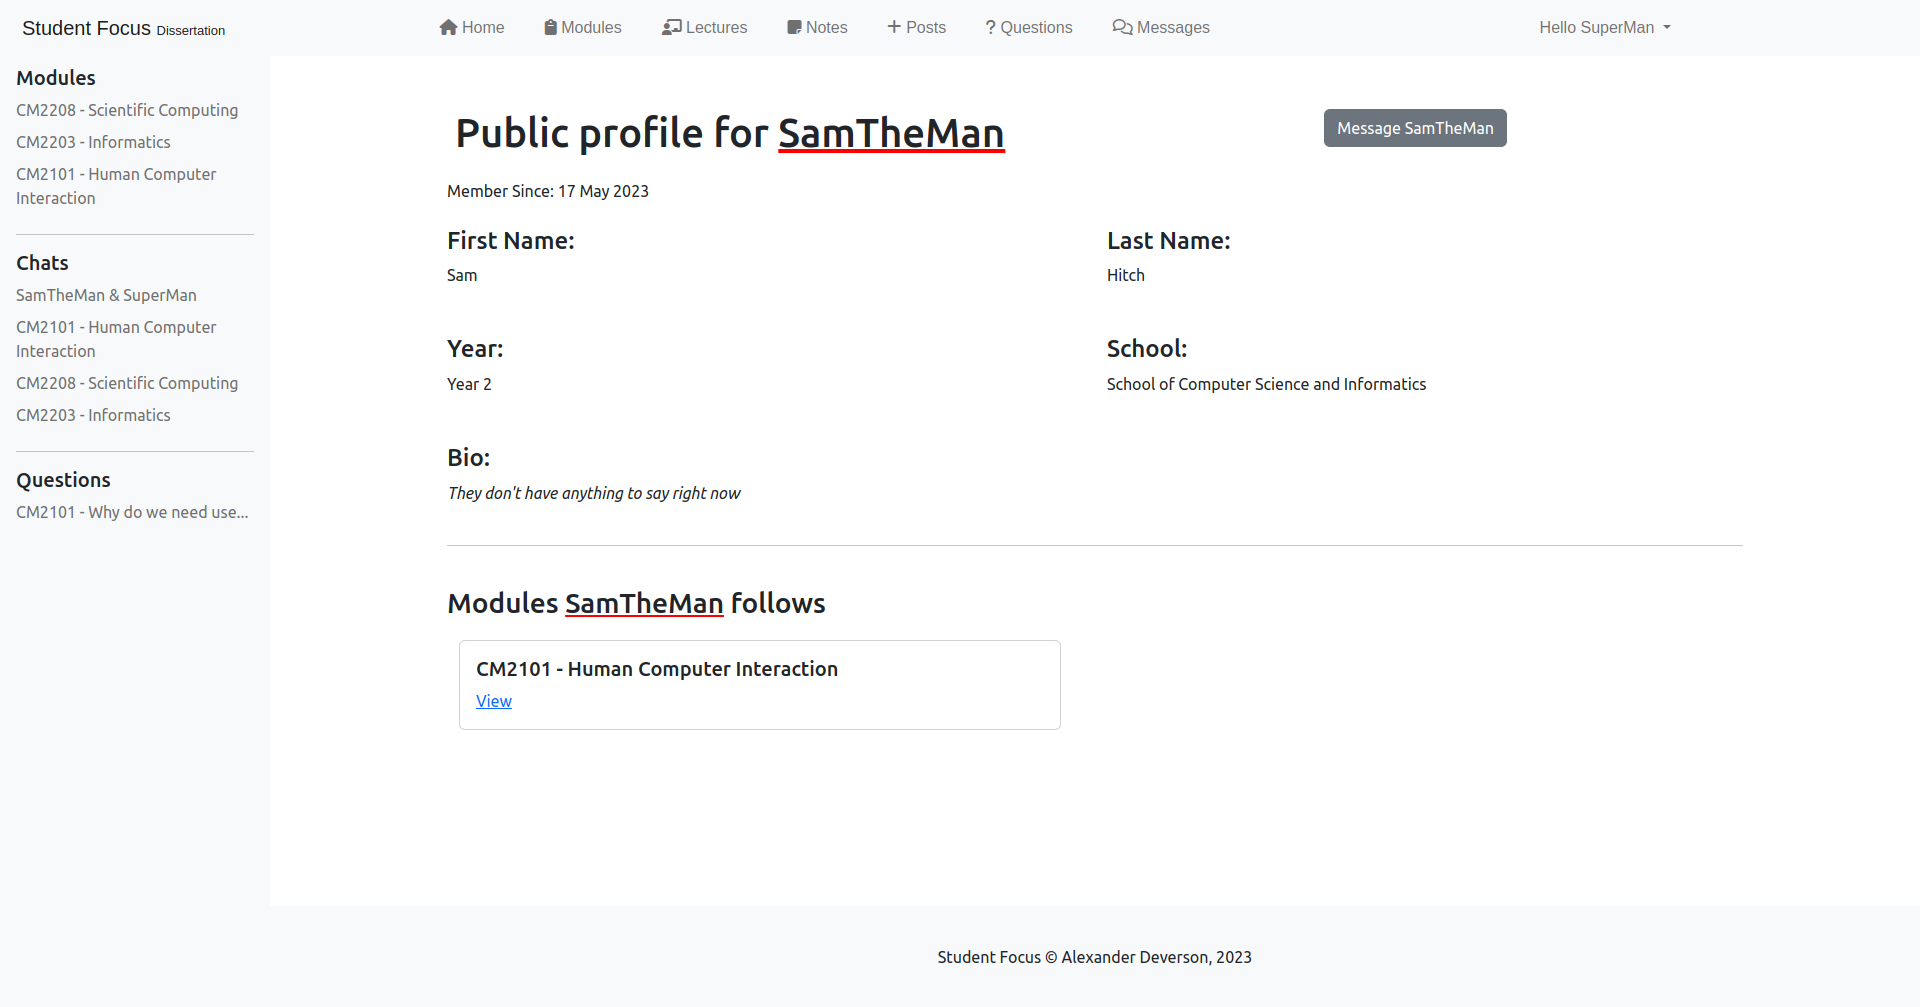
\includegraphics[scale=0.20]{images/application/27 - sams_profile.png}
\caption{Other user's profile page}
\label{fig:figure2}
\end{figure}

The user can view the profile of another user, seeing details about them and what modules they are taking.

\begin{figure}[H]
\centering
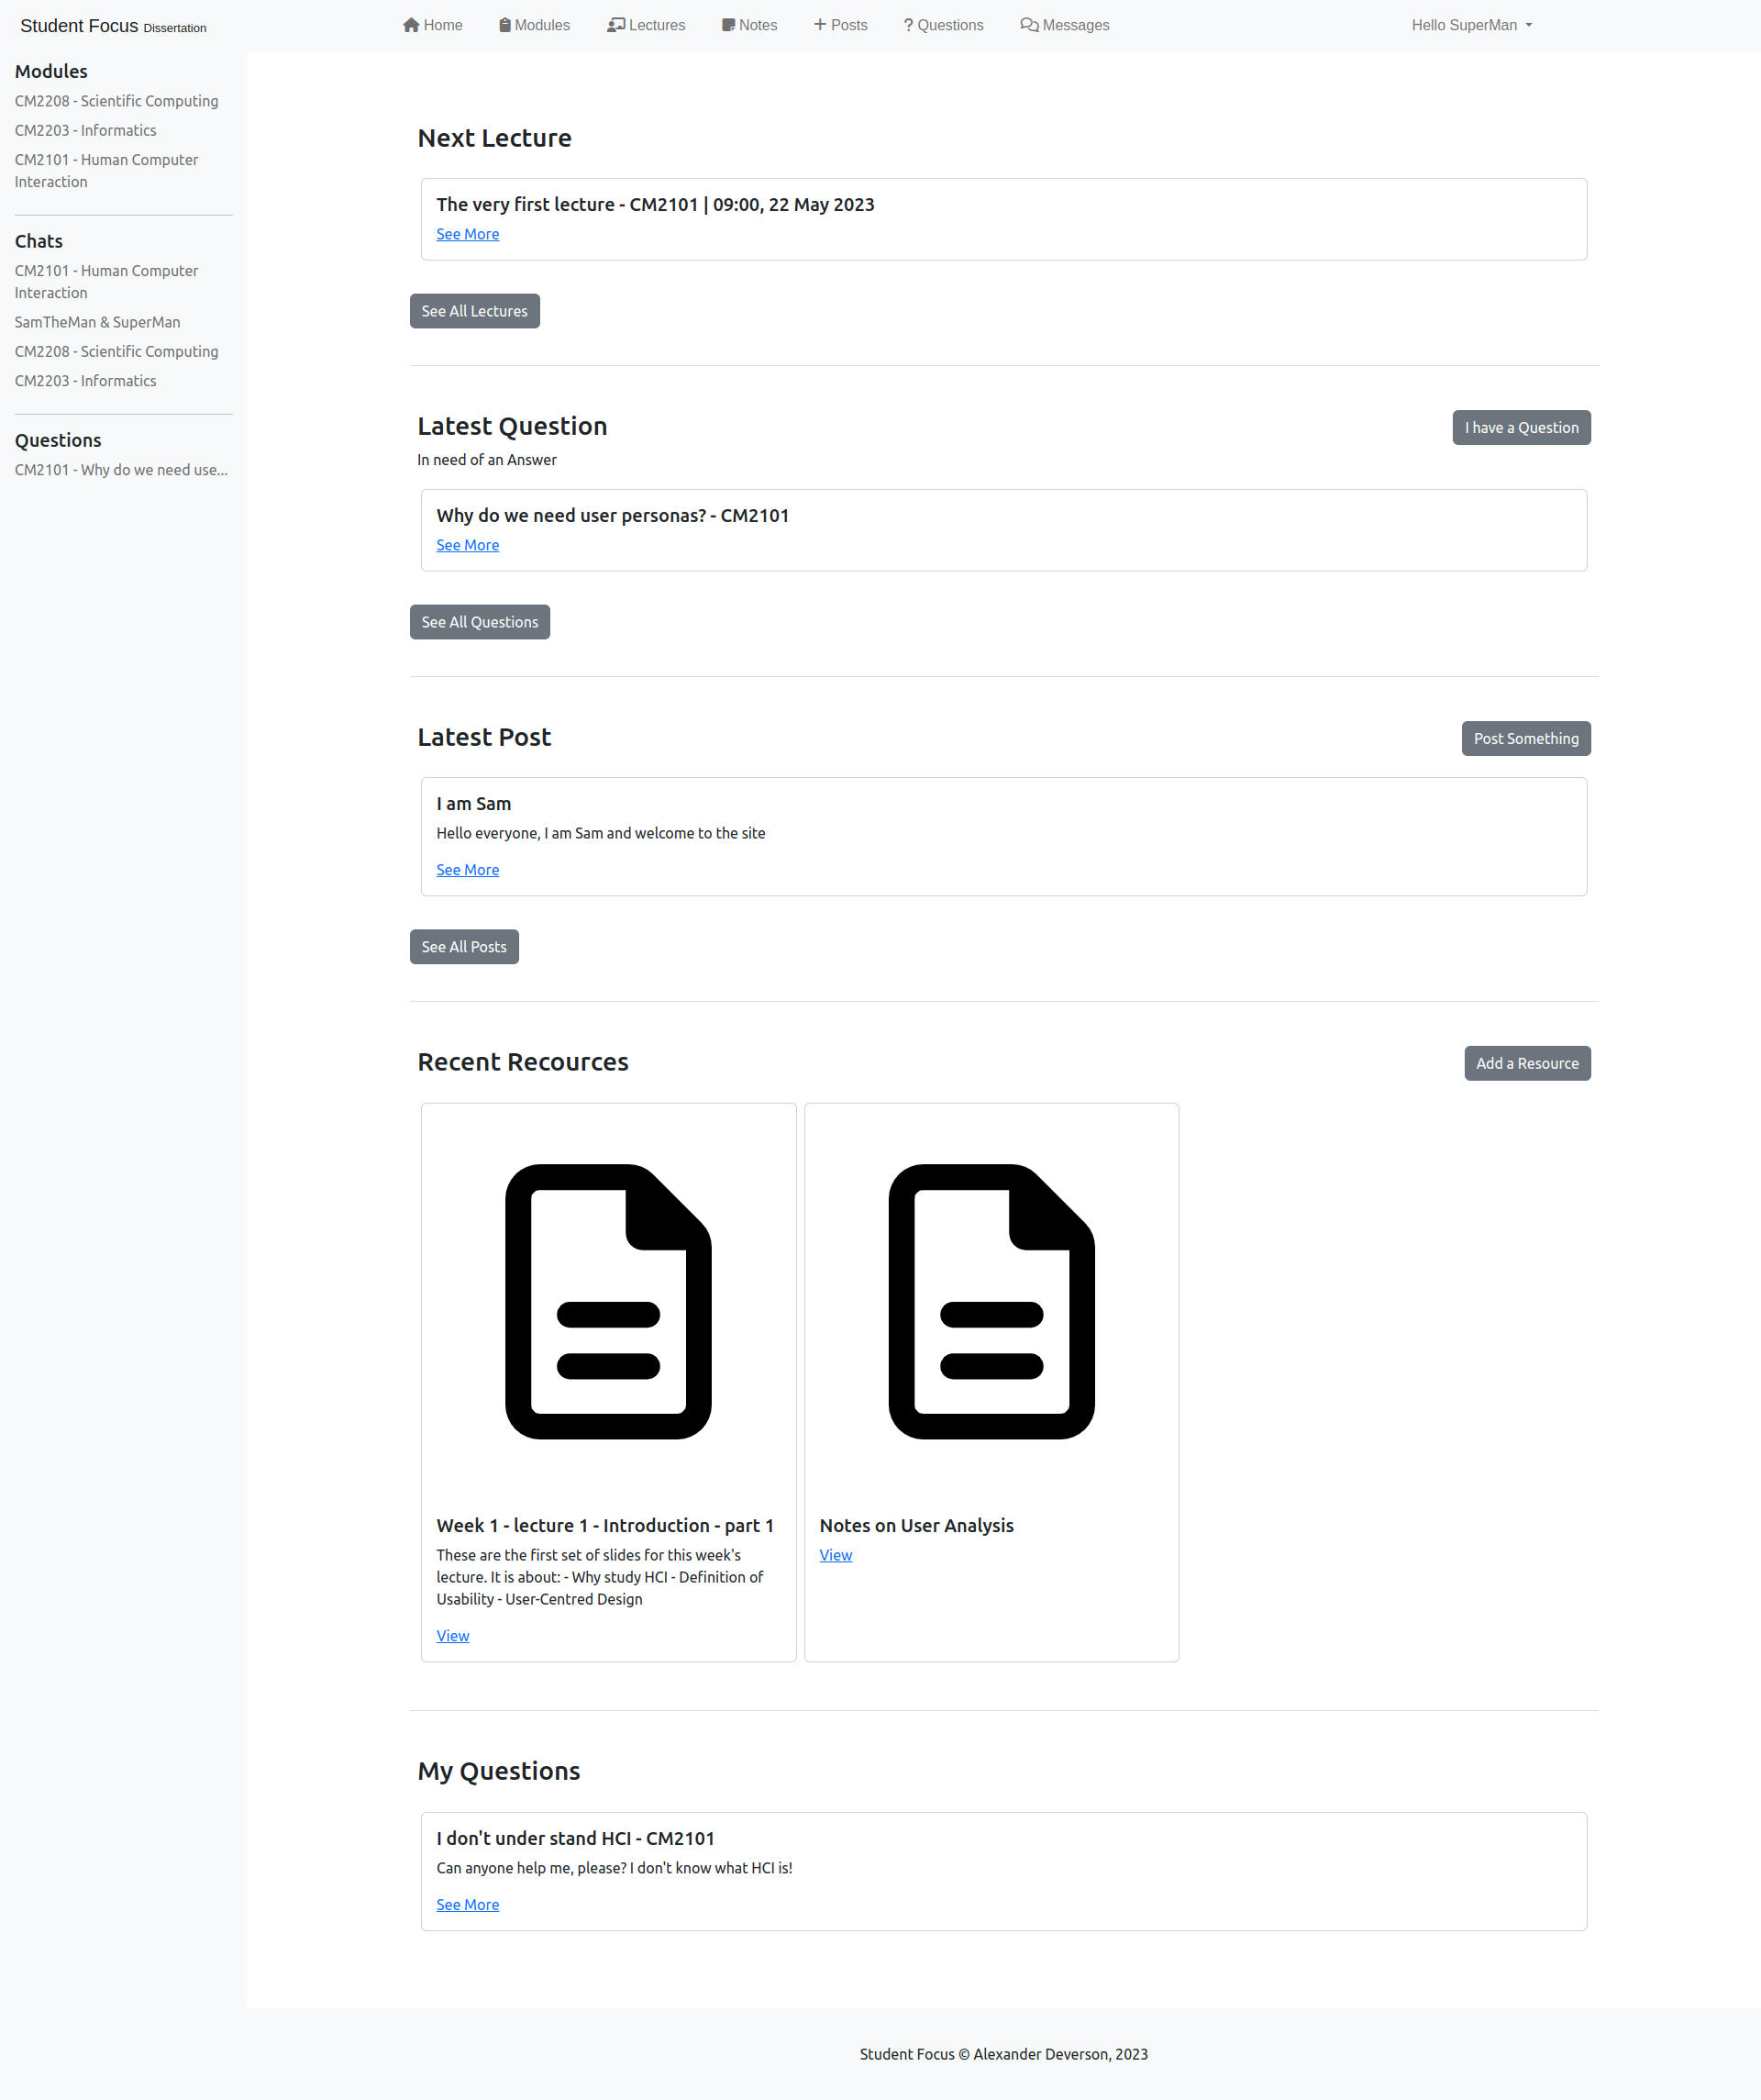
\includegraphics[scale=0.20]{images/application/34 - home_page_populated.png}
\caption{User's home page populated with content}
\label{fig:figure2}
\end{figure}

This shows how the main user home page will start to look after each section is populated with some content. Currently, for the resources, only documents have been uploaded to the site. If an image were uploaded, then it would show a preview of the image instead of an icon of a document. 

Here the user has quick access to all the essential things they may need to see. They can see recently uploaded module resources, the latest public post, the newest questing posted by a different user (the current user's question will never show under "latest question"), the next lecture from any module the user is subscribed to (regardless of how far into the future the lecture maybe) and at the bottom the user has quick access to any questions they have posted.

\begin{figure}[H]
\centering
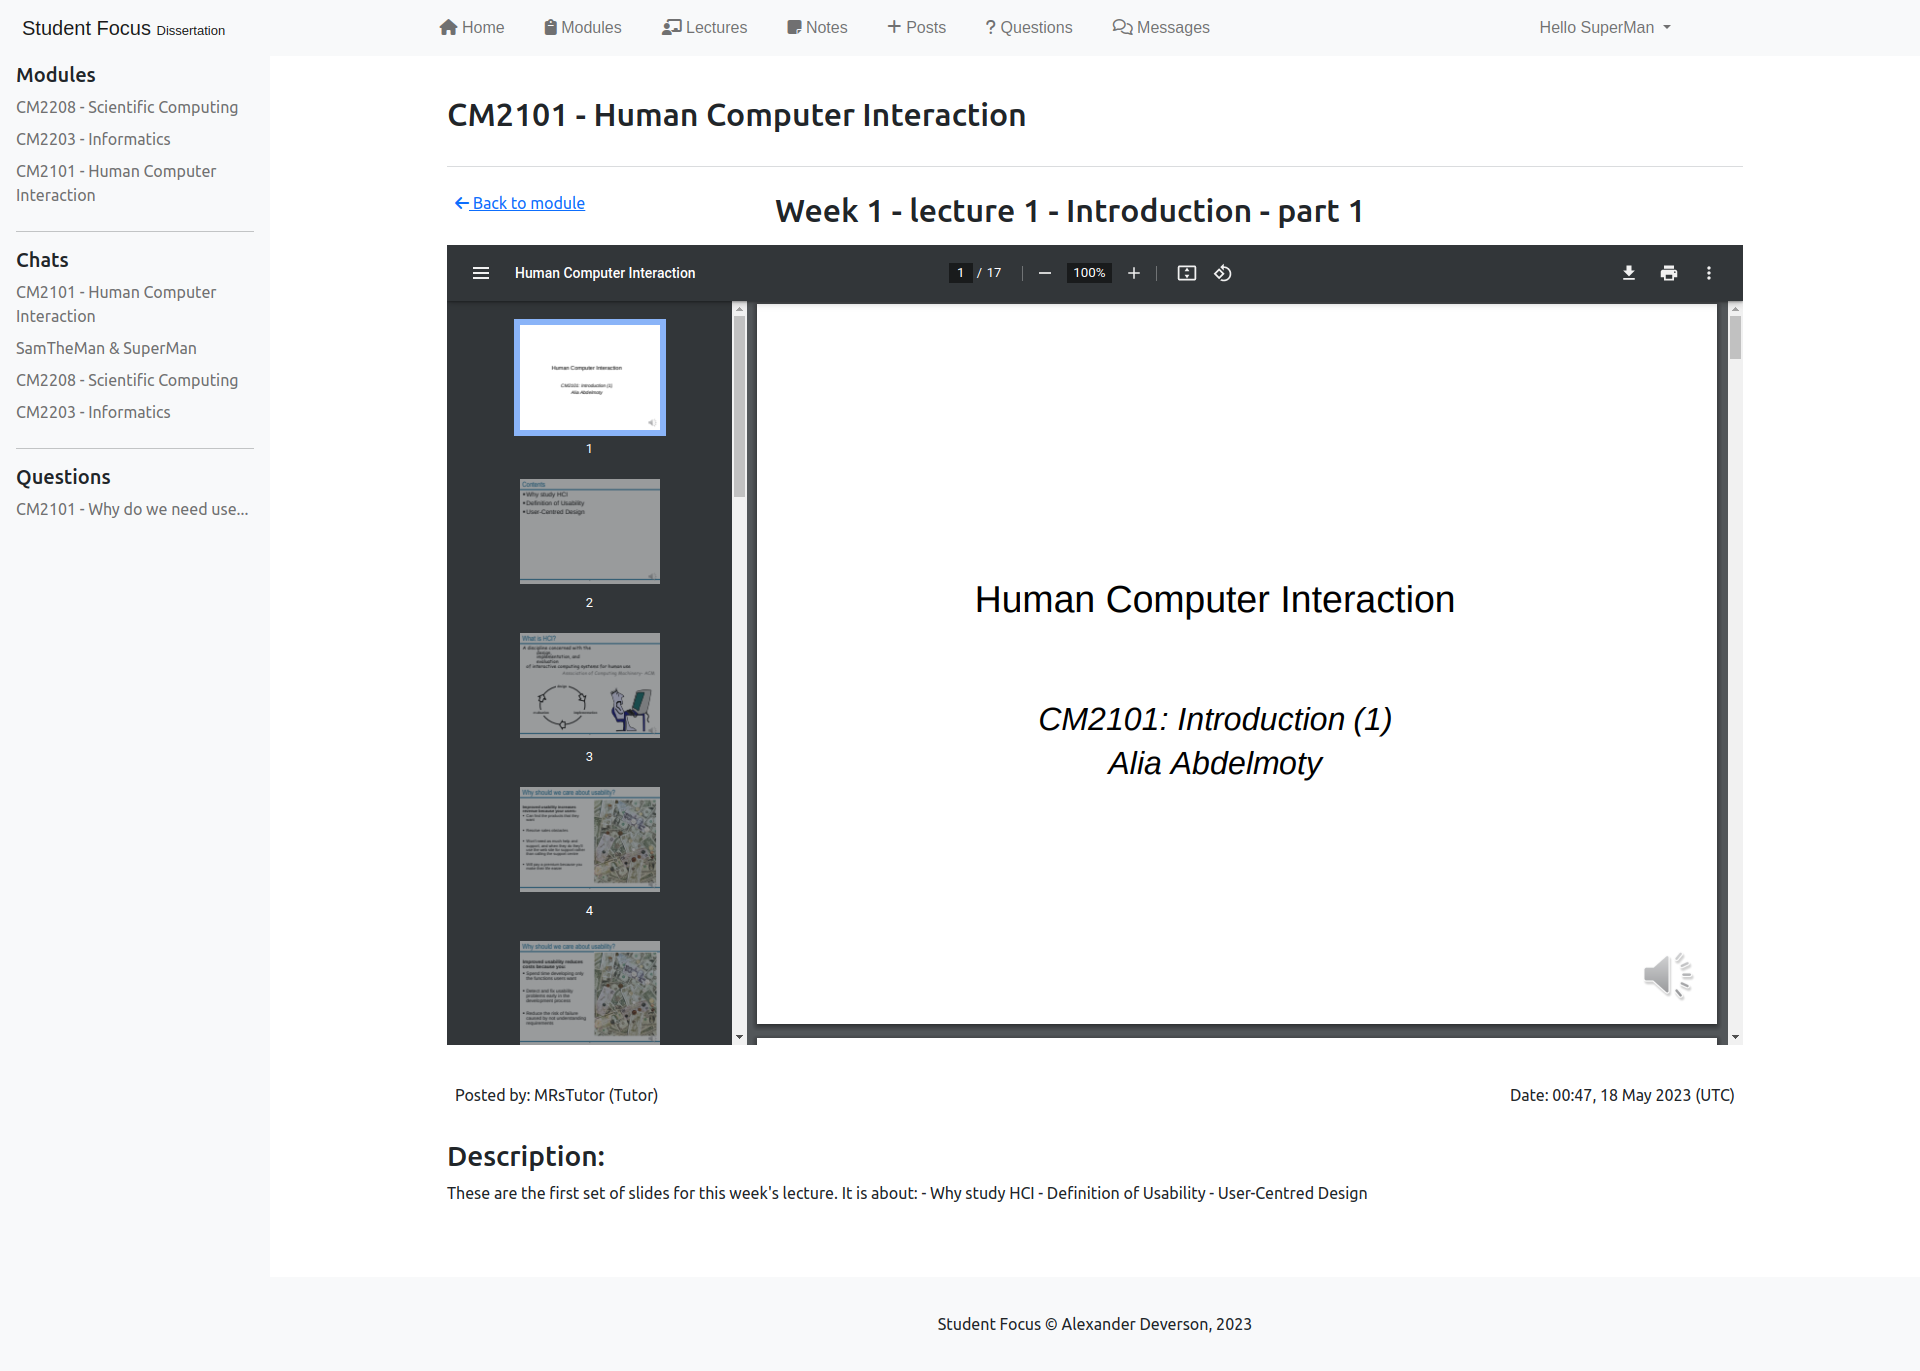
\includegraphics[scale=0.20]{images/application/35 - resource_single_view.png}
\caption{rResource single view}
\label{fig:figure2}
\end{figure}

This shows how a module resource will look after a user click on one to view its contents. Currently, a document is being shown, but an image resource with look the same. The difference is the pdf being shown would be replaced with the image. 

\begin{figure}[H]
\centering
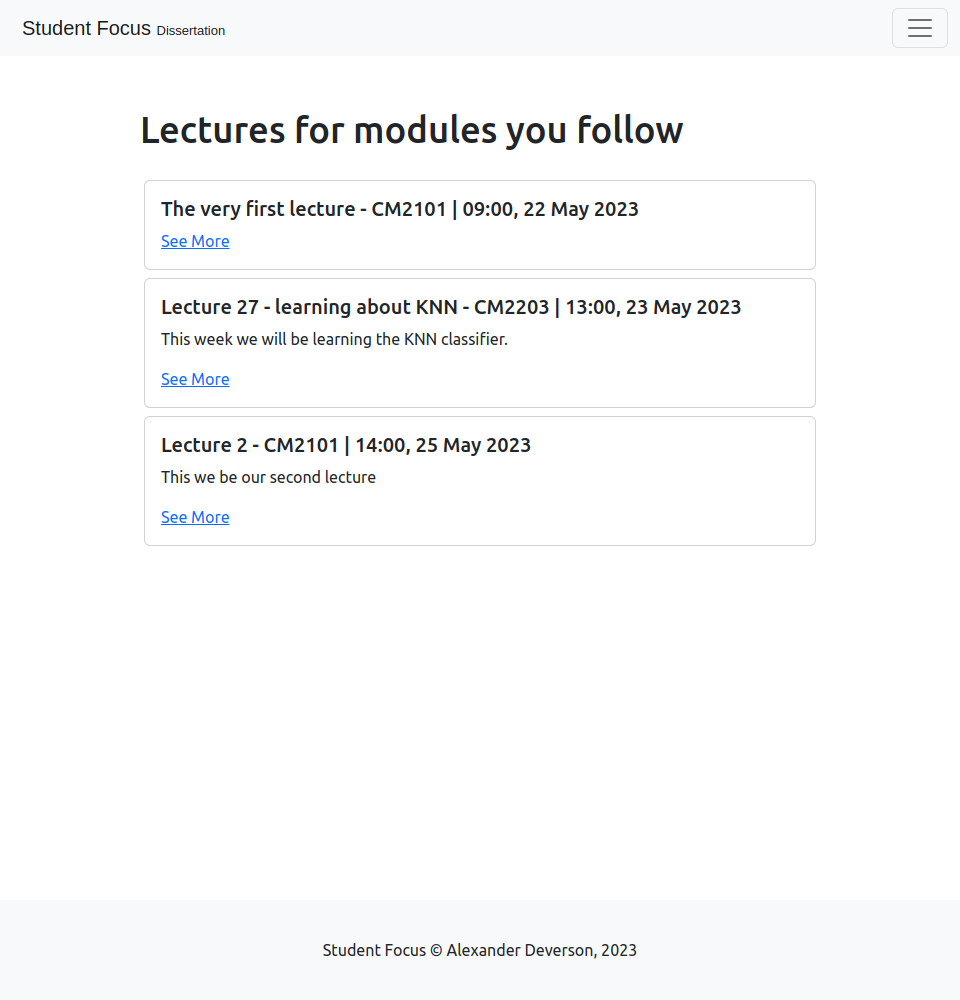
\includegraphics[scale=0.35]{images/application/38 - lecture_list_more.png}
\caption{List of all upcoming lectures}
\label{fig:figure2}
\end{figure}

This page shows a list of all the upcoming lectures for all the modules that a user has subscribed to. Lecture that have past the current date, will never be shown here.

\begin{figure}[H]
\centering
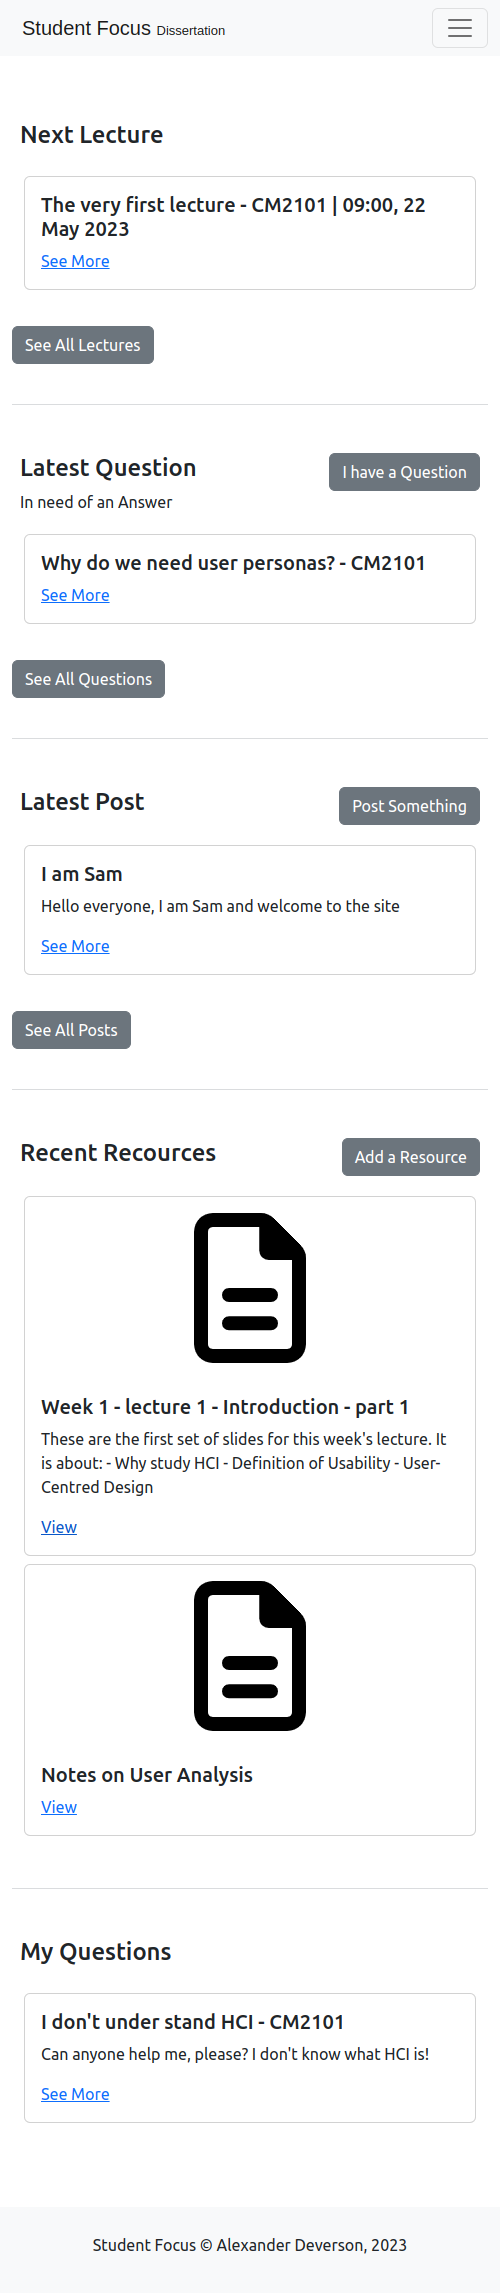
\includegraphics[scale=0.25]{images/application/44 - mobile_home.png}
\caption{Mobile view of the user's home page}
\label{fig:figure2}
\end{figure}

This shows a mobile version of the user's home page. As the application is built with a mobile-first philosophy, the elements will stack on top of each other to be easily viewable and readable on a mobile device.

\begin{figure}[H]
\centering
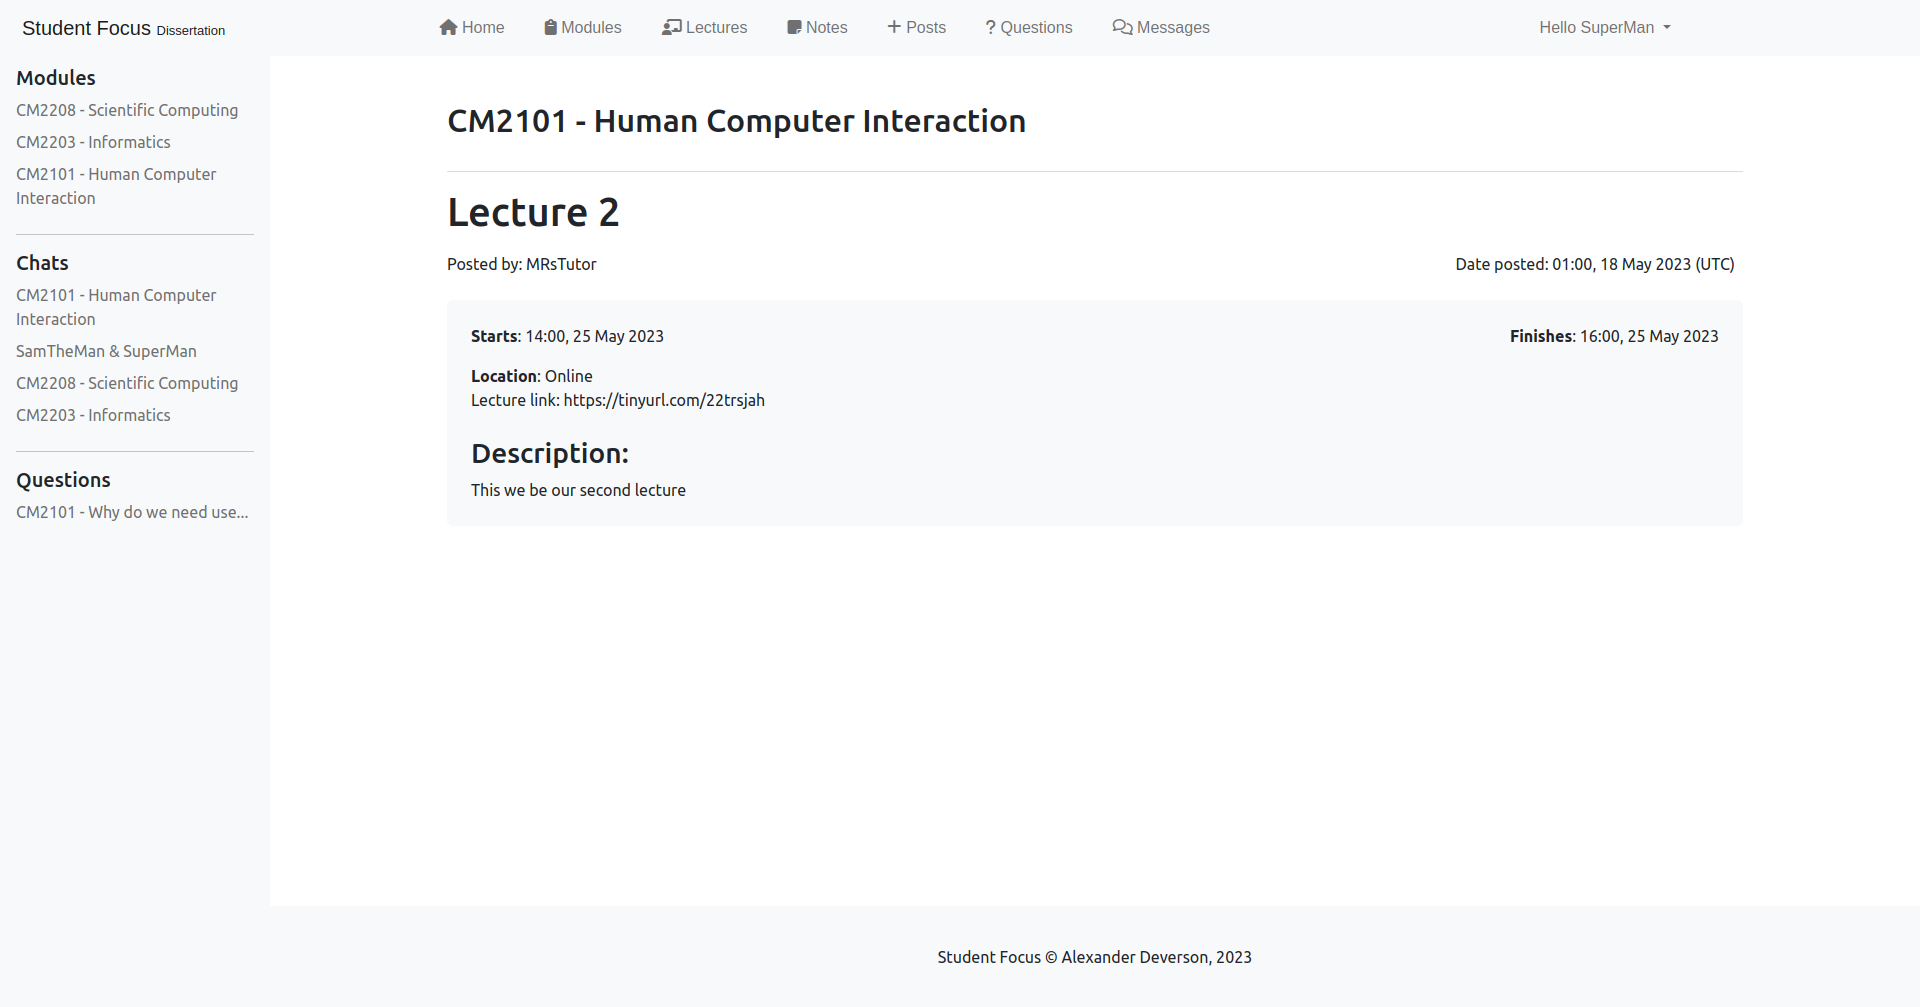
\includegraphics[scale=0.20]{images/application/45 - lecture_single.png}
\caption{Single lecture page view}
\label{fig:figure2}
\end{figure}

This shows how a single lecture page with look when a user clicks on a lecture to view more information.

\begin{figure}[H]
\centering
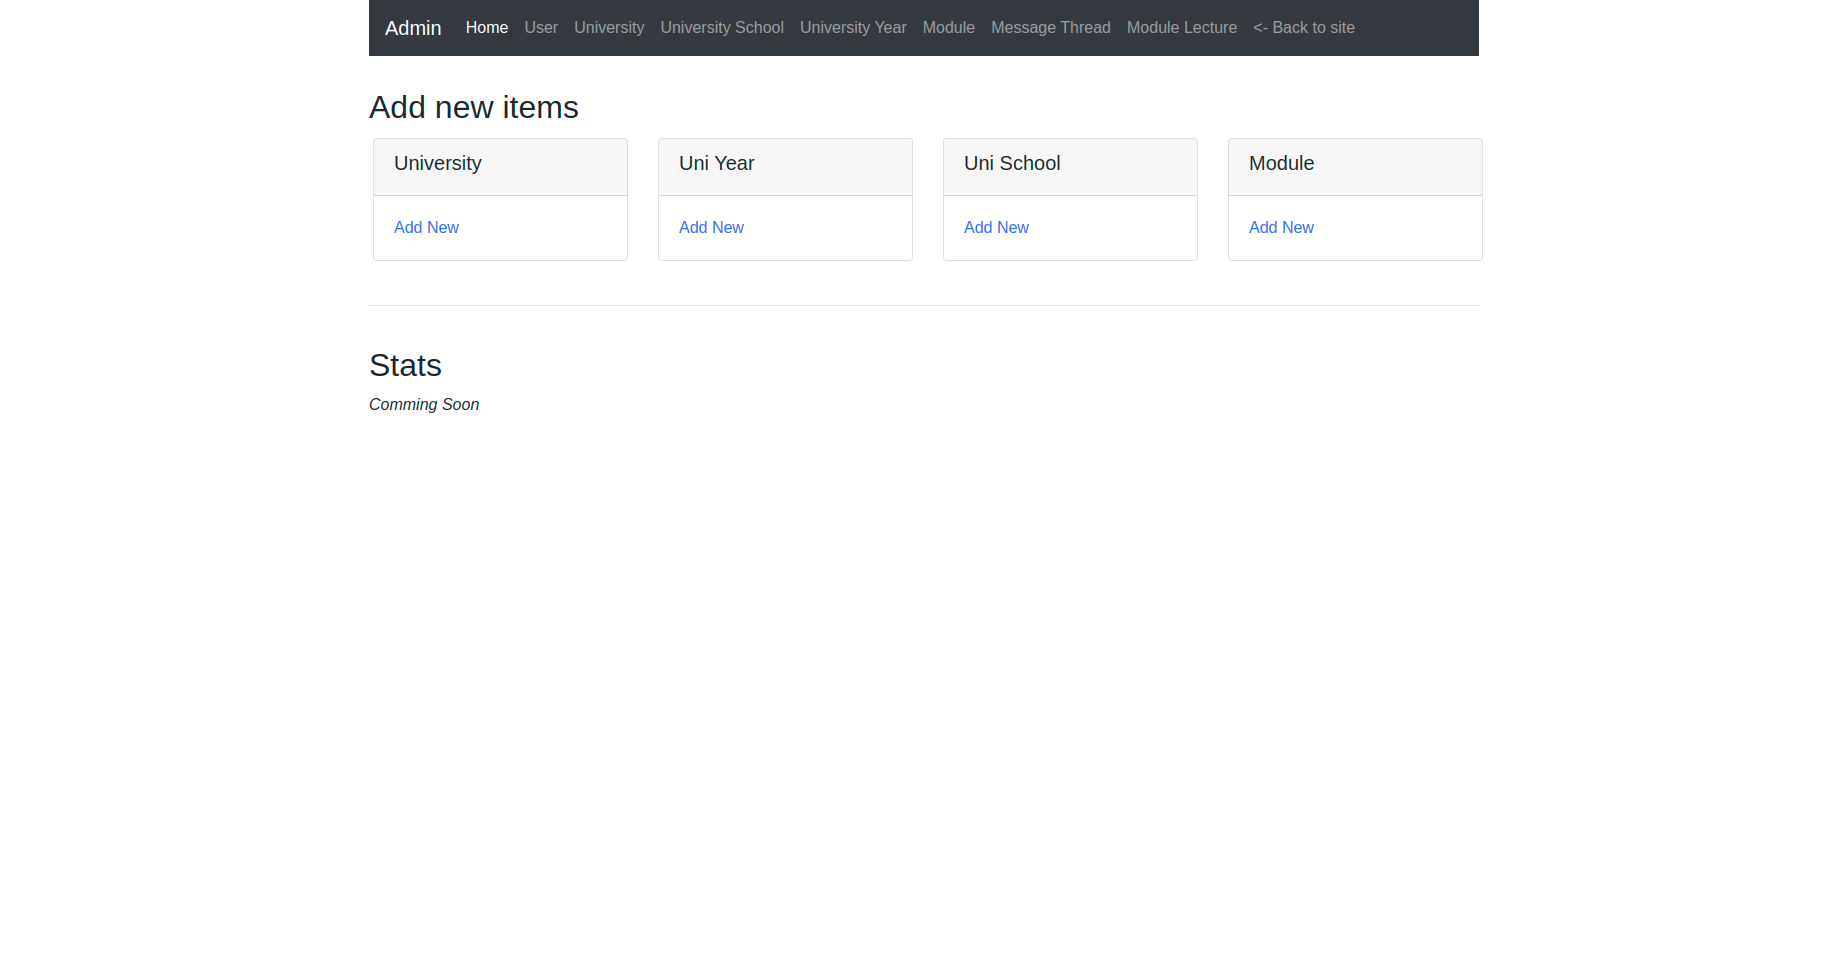
\includegraphics[scale=0.20]{images/application/48 - admin_home.png}
\caption{Admin home page view}
\label{fig:figure2}
\end{figure}

This shows the admin home page and what they have access to and can update or add.

\begin{figure}[H]
\centering
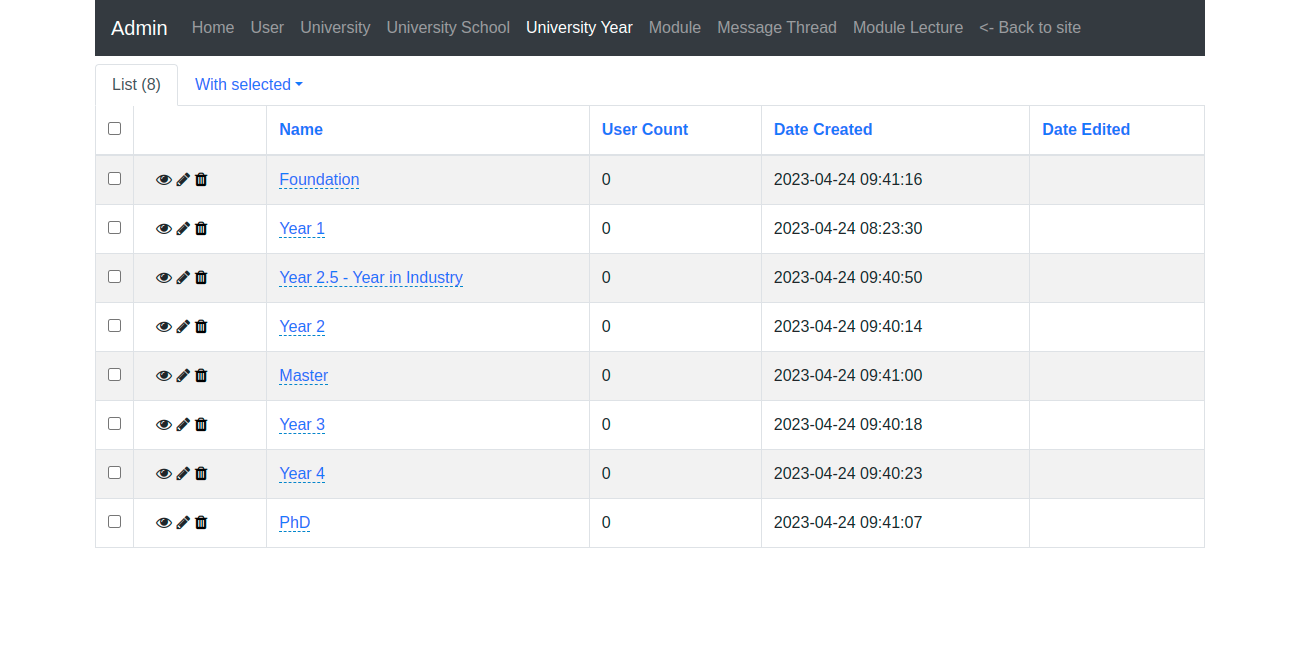
\includegraphics[scale=0.35]{images/application/49 - admin_table_example.png}
\caption{Admin table view}
\label{fig:figure2}
\end{figure}

This shows an example of one of the table pages from the top navigation. The table is currently showing the university year table.

\begin{figure}[H]
\centering
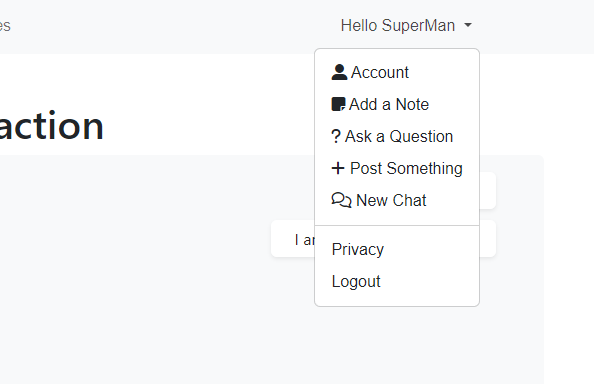
\includegraphics[scale=0.50]{images/application/55 - nav_user_dropdwon.png}
\caption{logged in User drop-down}
\label{fig:figure2}
\end{figure}

This shows the user navigation dropdown when they are logged into the application. The user has quick access to create any type of content available from any page in the application. They will be taken to the appropriate page once clicking on a link.

\begin{figure}[H]
\centering
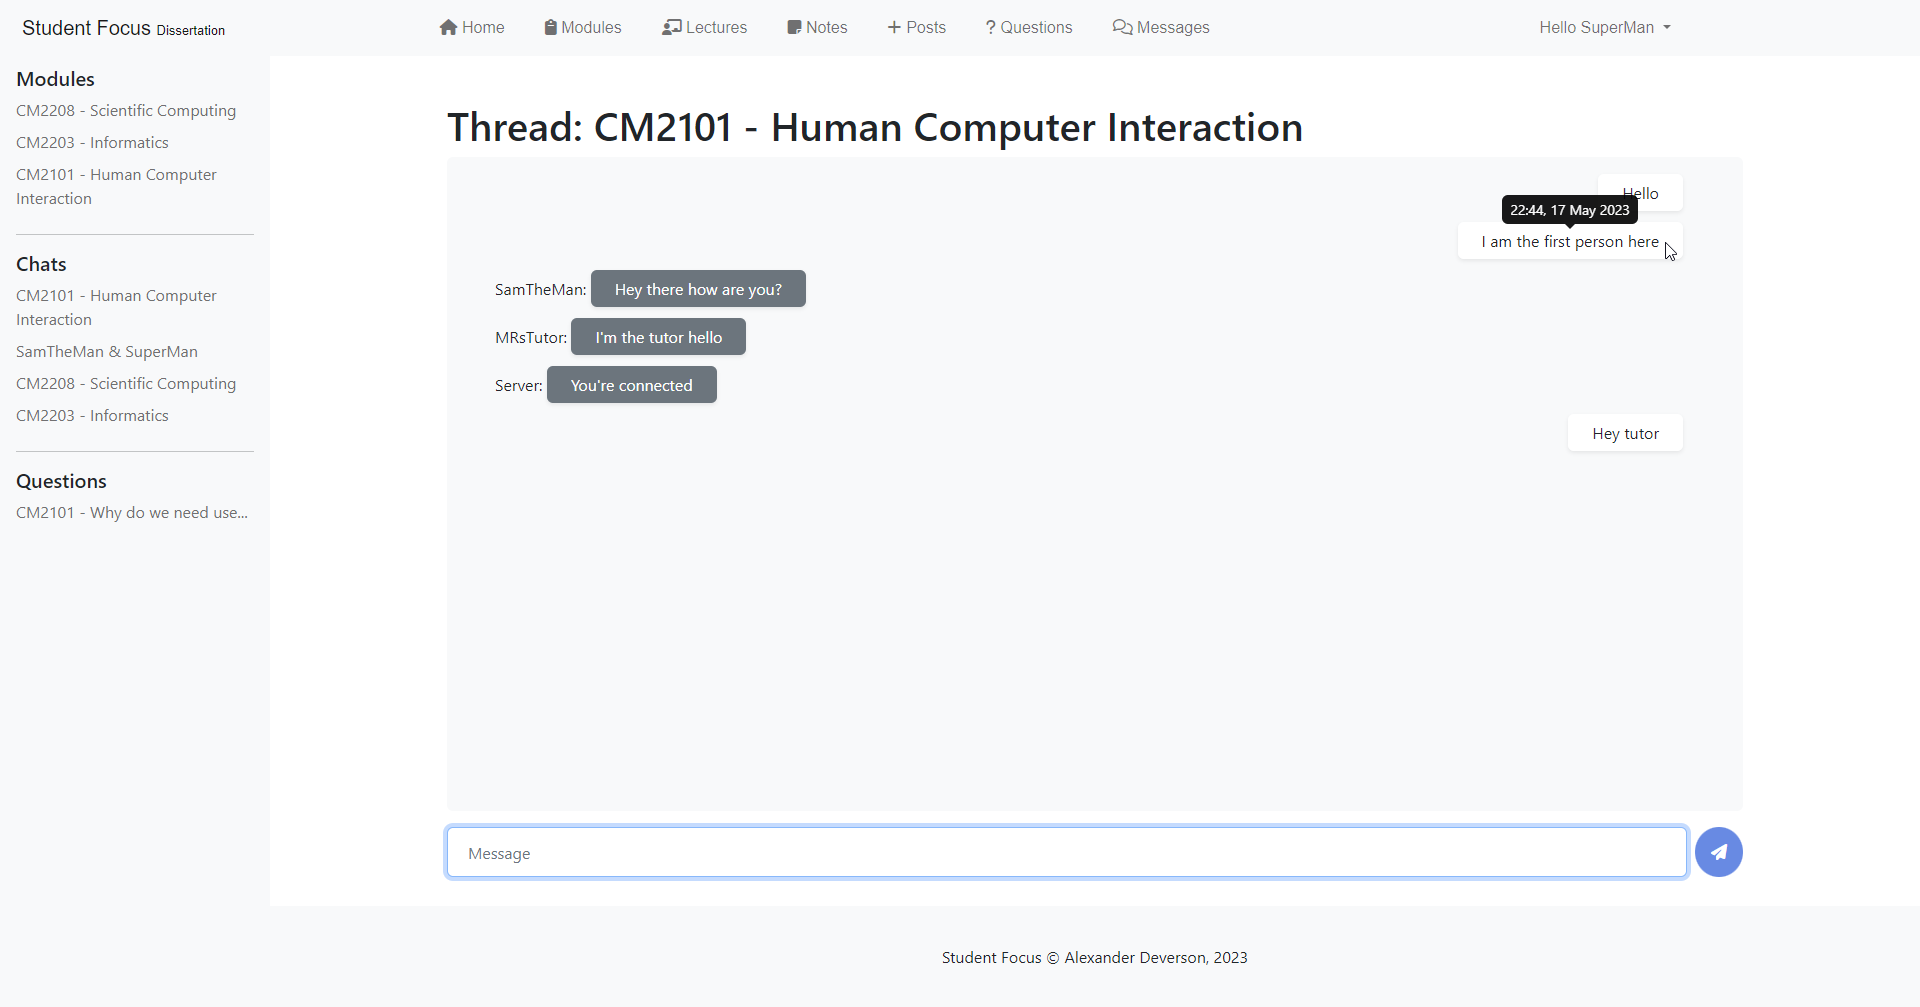
\includegraphics[scale=0.27]{images/application/59 - message_hover.png}
\caption{Showing the tooltips when a message is hovered over}
\label{fig:figure2}
\end{figure}

This shows the tooltips for when a user hovers over a message in the real-time chat section. This also works for messages on a single module page and for chats and questions in the sidebar. This is to allow the user to see extra information that may be useful but not necessary for continuous viewing. This simplifies the view of the application and makes it appear clean, tidy and more organised.

\begin{figure}[H]
\centering
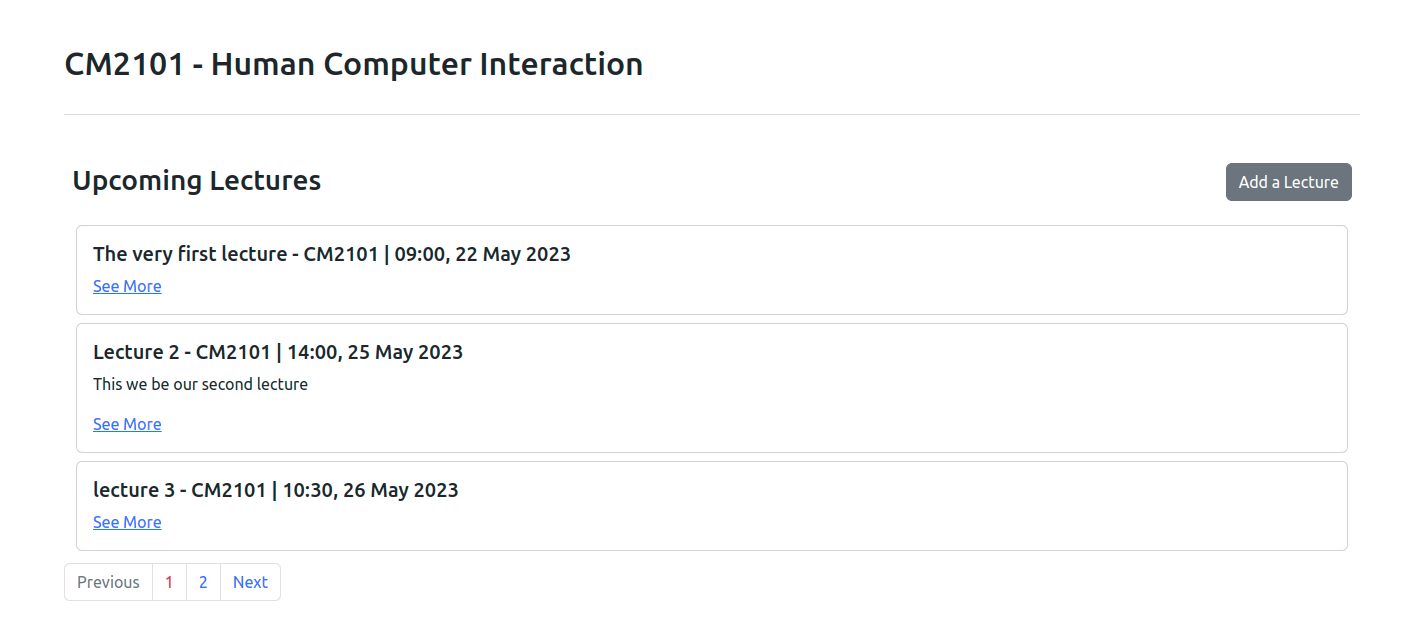
\includegraphics[scale=0.27]{images/application/64 - lectures.png}
\caption{Showing page pagination for lectures}
\label{fig:figure2}
\end{figure}

This is an example showing when there are too many items, such as for lectures, questions, posts, comments, etc, and they become paginated on to multiple pages so that too many are not loaded at once.

\begin{figure}[H]
\centering
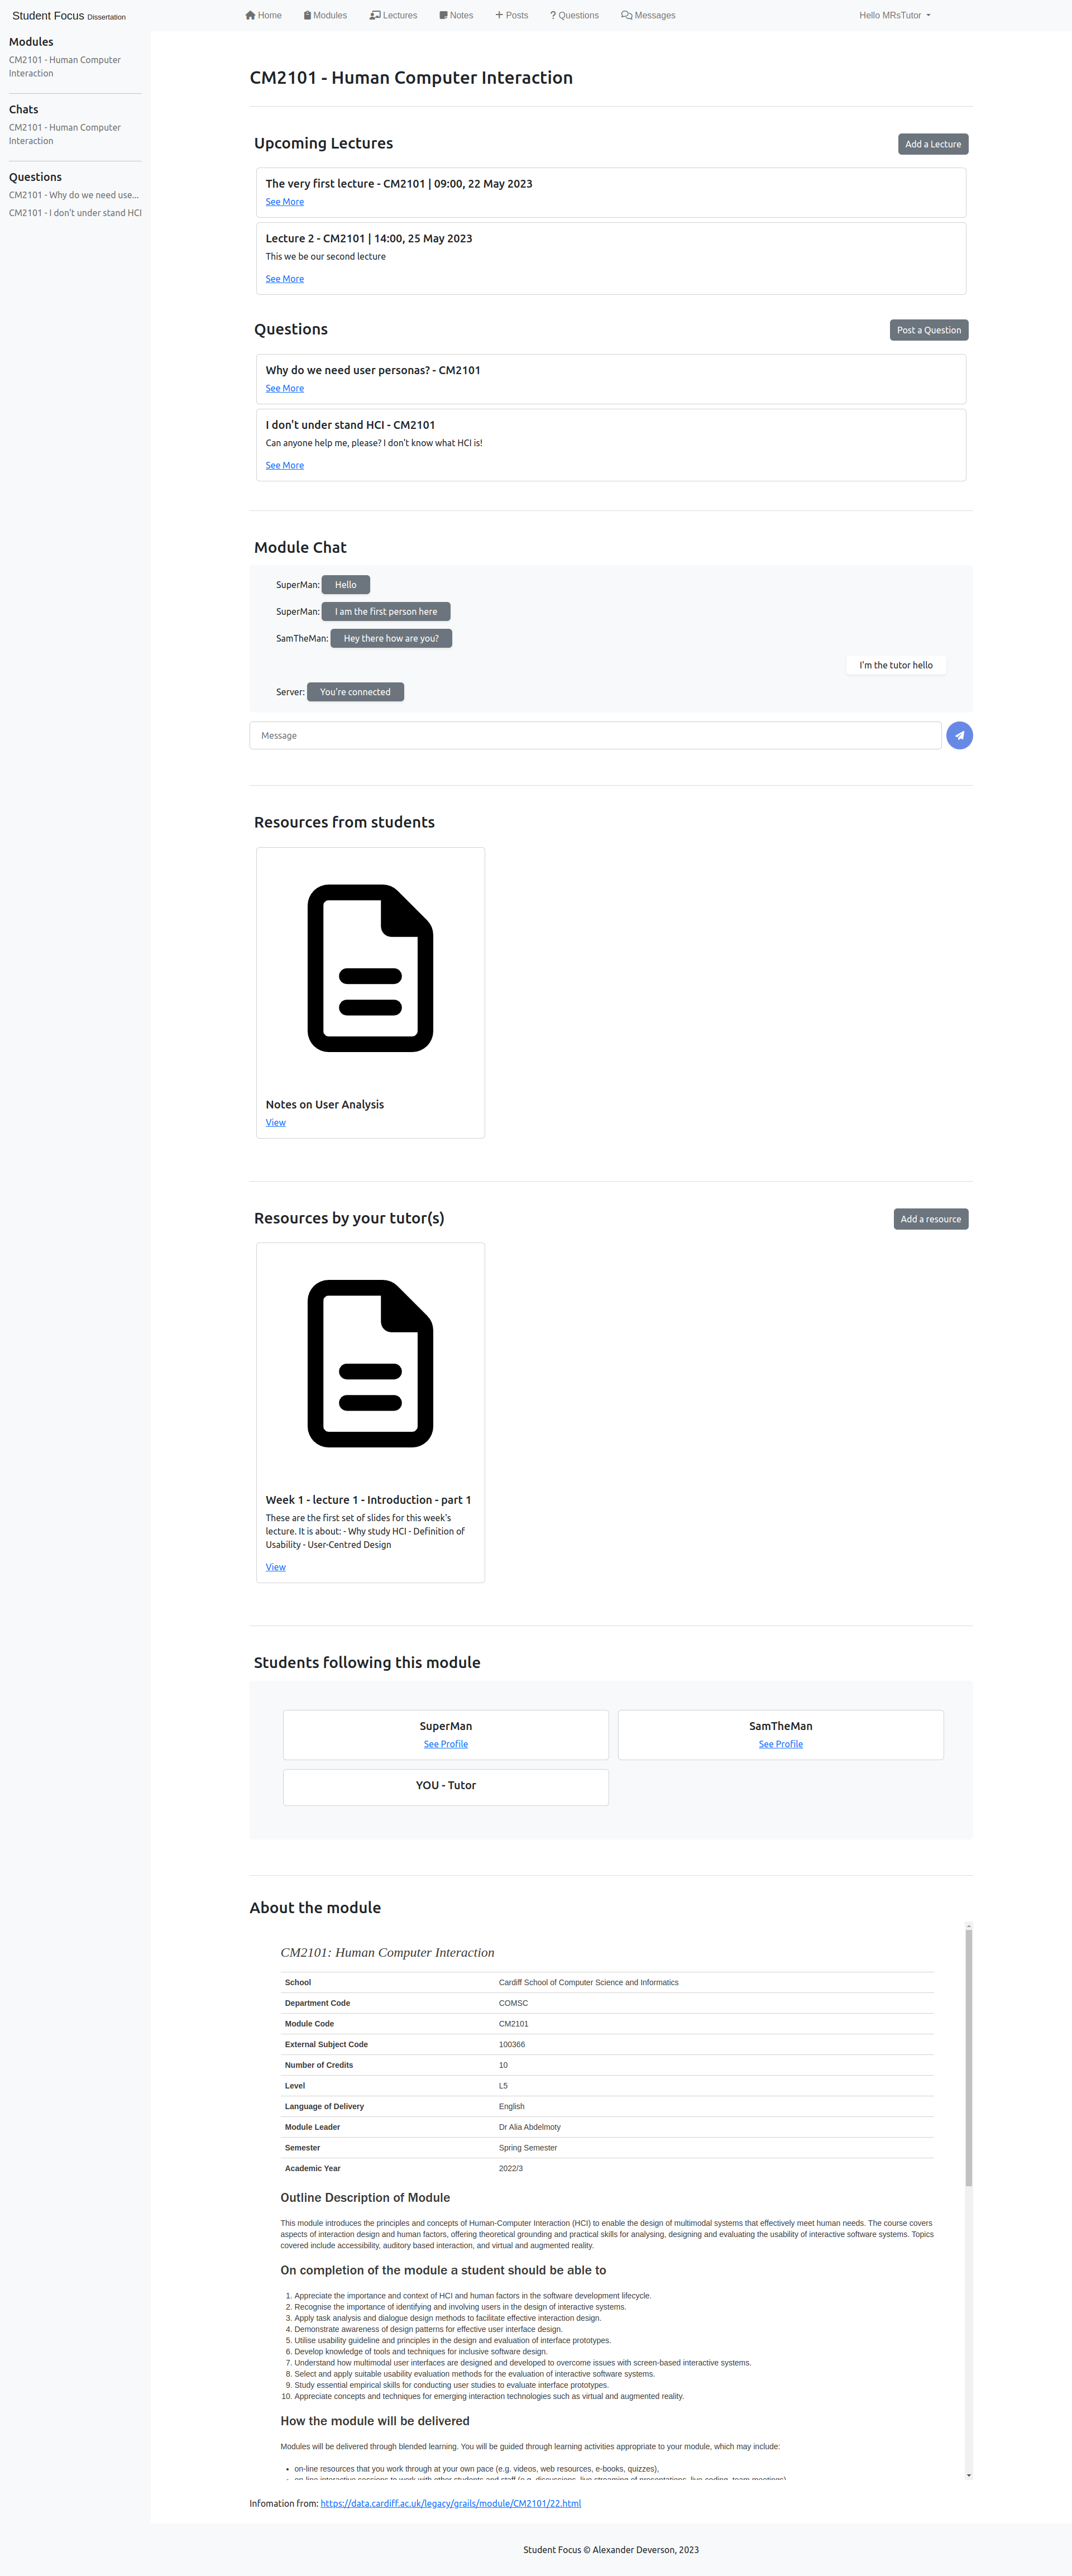
\includegraphics[scale=0.13]{images/application/36 - tutor_module_page_populated.png}
\caption{Populated single module page}
\label{fig:figure2}
\end{figure}

This is a view of a single module page  where all sections are populated from a tutor's perspective.
